\documentclass{article}

% Language setting
\usepackage[spanish]{babel}
\usepackage{amssymb,stackengine} 
\newcommand{\checkedbox}{\stackinset{c}{0pt}{c}{0pt}{\checkmark}{$\square$}}
\usepackage[letterpaper,top=2cm,bottom=5cm,left=3cm,right=3cm,marginparwidth=1.75cm]{geometry}

% Useful packages
\usepackage{amsmath}
\usepackage[utf8]{inputenc}
\usepackage{tabularx}
\usepackage{float}
\usepackage{geometry}
\geometry{margin=1in}
\usepackage{array}
\renewcommand{\arraystretch}{1.5}
\usepackage{graphicx}
\usepackage[colorlinks=true, allcolors=blue]{hyperref}
\usepackage{fancyhdr}
\usepackage{lipsum}
\usepackage{multicol}
\pagestyle{fancy} 
\usepackage[table]{xcolor}
\usepackage{booktabs}
\usepackage{titlesec}
\usepackage{longtable}
\usepackage{multirow}

\fancyhf{} % Limpiar encabezado y pie de página por defecto
\setlength{\headheight}{70pt} 

% Definición del encabezado
\fancyhead[C]{%
    \begin{minipage}[c]{2.5cm}
        \centering
        \includegraphics[width=2.2cm]{imagenes/uta.png}
    \end{minipage}%
    \hfill
    \begin{minipage}[c]{8cm} 
        \centering
        \small {\textbf{UNIVERSIDAD TÉCNICA DE AMBATO}} \\[0.1cm]
        \scriptsize \textit{FACULTAD DE INGENIERÍA EN SISTEMAS, ELECTRÓNICA E INDUSTRIAL} \\[0.1cm]
        \scriptsize \textbf{CARRERA DE SOFTWARE} \\[0.1cm]
        \scriptsize \textbf{CICLO ACADÉMICO: ENERO 2026 - JULIO 2026}
    \end{minipage}%
    \hfill
    \begin{minipage}[c]{2.5cm}
        \centering
        \includegraphics[width=2.2cm]{imagenes/fisei.png}
    \end{minipage}%
}

\begin{document}
\begin{center}
    {\large \textbf{INFORME DE GUÍA PRÁCTICA}} \\    
\end{center}

\section{Portada}
\begin{flushleft}
\begin{tabular}{ l l }
    \textbf{Tema:} & Desarrollo de Redes Neuronales MLP para Inteligencia de Negocios\\
    \textbf{Unidad de Organización Curricular:} & Profesional \\
    \textbf{Nivel:} & Sexto \\
    \textbf{Alumnos:}
                    & Josué Fiallos \\
                    & Marlon Guevara \\
                    
    \textbf{Asignatura:} & Inteligencia Artificial \\
    \textbf{Docente:} & Ing. Mg. Rubén Nogales \\
\end{tabular}
\end{flushleft}

\section{Informe de guía práctica}
\subsection{Objetivos}
\subsubsection{General}
Desarrollar, entrenar y evaluar modelos de Redes Neuronales Artificiales (Perceptrón Multicapa) para la predicción y toma de decisiones estratégicas en entornos empresariales, demostrando solidez matemática y técnica en el procesamiento de datos.

\subsubsection{Específicos}
\begin{itemize}
    \item Describir y contextualizar rigurosamente los cinco datasets empresariales del proyecto (\textit{fact\_ventas, fact\_inventario, fact\_competencia, fact\_abastecimiento\_logistica, fact\_evaluacion\_proveedores}), detallando sus variables de entrada, variable objetivo, distribución de muestras y el proceso de preprocesamiento aplicado (normalización por cuantiles y sobremuestreo para balanceo de clases).
    \item Fundamentar matemáticamente la arquitectura MLP: demostrar el cálculo de la combinación lineal de entrada $Z^{(l)} = W^{(l)}A^{(l-1)} + b^{(l)}$, el papel probabilístico de la función de activación Sigmoide en las capas ocultas, la normalización Softmax en la capa de salida y la regla de clasificación \textit{argmax}.
    \item Ejecutar un entrenamiento fuerte y auditable documentando la configuración completa de hiperparámetros, la actualización de pesos mediante el algoritmo Adam (gradiente descendente adaptativo con regularización L2) y el historial de pérdida y exactitud por época.
    \item Evidenciar un testeo robusto reportando métricas de pérdida y exactitud (\textit{Accuracy}) en los tres conjuntos: entrenamiento, validación y prueba, para los cinco modelos MLP desarrollados.
\end{itemize}

\subsection{Modalidad}
Presencial

\subsection{Tiempo de duración}
\textbf{Presenciales:} 12 \\
\textbf{No presenciales:} 0

\subsection{Listado de equipos, materiales y recursos}
\textbf{Listado de equipos y materiales generales empleados en la guía práctica:}
\begin{itemize}
    \item Computadora e Internet
    \item Entorno de desarrollo (Jupyter Notebook, VSCode, Python)
\end{itemize}

\textbf{TAC (Tecnologías para el Aprendizaje y Conocimiento) empleados en la guía práctica:}
\begin{itemize}
    \item[$\blacksquare$] Plataformas educativas
    \item[$\blacksquare$] Simuladores y laboratorios virtuales (Flask Dashboard)
    \item[$\blacksquare$] Bases de datos de la biblioteca virtual
    \item[$\square$] Recursos audiovisuales
    \item[$\blacksquare$] Inteligencia Artificial (Scikit-learn, Pandas)
    \item Otros: Framework de Dashboards web para despliegue. 
\end{itemize}

\subsection{Instrucciones}
Desarrollar una aplicación de Inteligencia Artificial que procese conjuntos de datos empresariales (Ventas, Logística, etc.) para realizar predicciones multiclase, asegurando un profundo nivel de análisis técnico según los siguientes puntos de rúbrica:
\begin{enumerate}
    \item \textbf{Análisis de Datos:} Describir el dataset y prepararlo.
    \item \textbf{Fundamento Matemático:} Definir la combinación lineal y el papel probabilístico de la función sigmoide.
    \item \textbf{Entrenamiento Fuerte:} Explicar la actualización por gradiente descendente, registrando hiperparámetros e historial.
    \item \textbf{Testeo Robusto:} Presentar métricas en entrenamiento, validación y prueba.
\end{enumerate}

\subsection{Resultados obtenidos}
A continuación, se detalla el cumplimiento técnico de los parámetros del modelo, integrando el preprocesamiento, el fundamento matemático simplificado y los resultados reales obtenidos en cada uno de los 5 hechos estratégicos del negocio.

\subsubsection{Preprocesamiento y Preparación de los Datos (Rúbrica: Análisis de Datos)}
Antes de entrenar la red neuronal, es indispensable limpiar y preparar los datos. En nuestro proyecto, se aplicaron dos procesos fundamentales de forma secuencial sobre los 5 conjuntos de datos (\textit{Ventas, Inventario, Competencia, Abastecimiento y Proveedores}):
\begin{itemize}
    \item \textbf{Transformación por Cuantiles (\textit{QuantileTransformer}):} 
    \textit{En palabras sencillas:} Las variables de negocio vienen en escalas muy diferentes (por ejemplo, el volumen de stock puede ser de miles de unidades, mientras que el descuento es un porcentaje entre 0 y 1). Si ingresamos estos datos directamente, la red neuronal le daría más importancia al stock simplemente por tener números más grandes. La transformación por cuantiles toma estas variables y las mapea uniformemente a una escala estándar, eliminando el efecto de valores extremos o atípicos.
    
    \textit{Matemáticamente:} Se calcula mapeando cada característica continua $x$ mediante su función de distribución acumulada (CDF) empírica $F(x)$ y la función cuantil $G^{-1}$ de la distribución objetivo:
    \begin{equation}
        x' = G^{-1}(F(x))
    \end{equation}
    Donde $G^{-1}$ es la función cuantil de la distribución objetivo y $F(x)$ es la CDF de la característica original.

    \item \textbf{Sobremuestreo (Oversampling):}
    \textit{En palabras sencillas:} En la realidad de la empresa, hay eventos muy comunes (por ejemplo, transacciones con "Stock Normal") y eventos muy raros (como "Quiebre de Stock"). Si entrenamos la red con este desbalance, la red aprendería a predecir siempre "Normal" para tener una precisión aparentemente alta. El sobremuestreo duplica de forma inteligente los ejemplos raros en el conjunto de entrenamiento para que la red aprenda a identificarlos por igual.
\end{itemize}

\subsubsection{Fundamento Matemático del Perceptrón Multicapa (MLP)}
El Perceptrón Multicapa es una red neuronal artificial estructurada en capas (capa de entrada, capas ocultas y capa de salida). Su funcionamiento se basa en tres operaciones clave:

\paragraph{1. Combinación Lineal y Parámetros (Rúbrica: Combinación Lineal)}
\textit{En palabras sencillas:} Cada neurona calcula un "promedio ponderado" de los datos que recibe. Multiplica cada entrada por un peso sináptico ($W$), que representa qué tan importante es esa variable, y le suma un sesgo o desviación ($b$), que ayuda a desplazar la decisión hacia arriba o hacia abajo. Esta operación calcula el potencial de activación de la neurona.

\textit{Matemáticamente:} Para una capa $l$, la combinación lineal pre-activación se calcula como:
\begin{equation}
    Z^{(l)} = W^{(l)} A^{(l-1)} + b^{(l)}
\end{equation}
Donde:
\begin{itemize}
    \item $A^{(0)} = X \in \mathbb{R}^{D}$ es el vector de entrada con $D$ características.
    \item $W^{(l)} \in \mathbb{R}^{n_l \times n_{l-1}}$ es la matriz de pesos que conecta la capa anterior con la capa actual $l$.
    \item $b^{(l)} \in \mathbb{R}^{n_l}$ es el vector de sesgo (bias) de la capa $l$.
\end{itemize}

\paragraph{2. Función de Activación Oculta (Rúbrica: Papel Probabilístico de la Sigmoide)}
\textit{En palabras sencillas:} La combinación lineal puede dar como resultado números muy grandes o muy pequeños. Para que la neurona decida si debe activarse y transmitir la información, aplicamos la función \textbf{Sigmoide} ($\sigma$). Esta función toma cualquier número y lo "aplasta" estrictamente a un valor entre 0 y 1, actuando como un interruptor de probabilidad (0 significa apagado, 1 encendido, y valores intermedios representan la certeza de activación). Al hacer esto en paralelo en cada neurona oculta, la red actúa como un banco de detectores de patrones complejos no lineales.

\textit{Matemáticamente:} La activación en las capas ocultas se rige por:
\begin{equation}
    a_j^{(l)} = \sigma\!\left(z_j^{(l)}\right) = \frac{1}{1 + e^{-z_j^{(l)}}}
\end{equation}
La sigmoide es diferenciable en todo su dominio, lo que permite que el error del modelo viaje hacia atrás durante el entrenamiento. Su derivada se calcula directamente usando su propia salida: $\sigma'(z) = \sigma(z)(1 - \sigma(z))$.

\paragraph{3. Capa de Salida y Regla de Decisión (Rúbrica: Regla de Clasificación)}
\textit{En palabras sencillas:} Dado que nuestros modelos deben clasificar los datos en 3 niveles de negocio (por ejemplo, Baja, Estándar o Alta rentabilidad), la capa de salida utiliza la función \textbf{Softmax} para repartir un "100\% de probabilidad" de forma proporcional entre las 3 clases. Finalmente, la regla de clasificación selecciona la clase con la probabilidad más alta mediante la función \textit{argmax}.

\textit{Matemáticamente:} Para la capa final $L$, la probabilidad estimada para cada clase $i$ y la predicción final $\hat{y}$ se definen como:
\begin{equation}
    a_i^{(L)} = P(y = i \mid X) = \frac{e^{z_i^{(L)}}}{\displaystyle\sum_{k=1}^{C} e^{z_k^{(L)}}}, \quad \hat{y} = \operatorname*{argmax}_{c \in \{0, 1, 2\}} \; a_c^{(L)}
\end{equation}
Donde $C = 3$ es el número de clases de salida.

\subsubsection{Optimización y Entrenamiento de la Red (Rúbrica: Gradiente Descendente)}
\textit{En palabras sencillas:} Entrenar la red neuronal significa ajustar los pesos ($W$) y sesgos ($b$) para minimizar los errores. La función de pérdida (Entropía Cruzada Categórica) mide qué tan lejos están las predicciones de la red de la realidad. El gradiente descendente es el método para ajustar estos parámetros: es como descender una montaña con niebla guiándose por la pendiente del terreno.

Para este proyecto se utilizó el algoritmo avanzado \textbf{Adam}, el cual ajusta automáticamente la velocidad de aprendizaje (tasa de aprendizaje) para cada peso de forma individual. Si un peso cambia de forma brusca, Adam reduce sus pasos para no pasarse del mínimo; si cambia muy lentamente, acelera el paso para aprender más rápido. Además, se aplicó la regularización L2 ($\lambda = 0.001$), que penaliza pesos excesivamente grandes para evitar que el modelo memorice los datos de entrenamiento (sobreajuste).

\textit{Matemáticamente:} La función de pérdida regularizada es:
\begin{equation}
    \mathcal{L}(W, b) = -\frac{1}{N} \sum_{n=1}^{N} \sum_{c=1}^{C} y_{n,c} \ln\!\left(a_{n,c}^{(L)}\right) + \frac{\lambda}{2N} \sum_{l=1}^{L} \sum_{j,k} \!\left(w_{j,k}^{(l)}\right)^{\!2}
\end{equation}
Y las ecuaciones de actualización del optimizador Adam en cada paso $t$ corresponden a:
\begin{align}
    g_t &= \nabla_{\theta}\, \mathcal{L}(\theta_t) \tag{Gradiente del error}\\
    m_t &= \beta_1 m_{t-1} + (1 - \beta_1)\, g_t \tag{Promedio móvil de gradientes}\\
    v_t &= \beta_2 v_{t-1} + (1 - \beta_2)\, g_t^2 \tag{Promedio móvil de varianza}\\
    \hat{m}_t &= \frac{m_t}{1 - \beta_1^t}, \qquad \hat{v}_t = \frac{v_t}{1 - \beta_2^t} \tag{Corrección de sesgo inicial}\\
    \theta_{t+1} &= \theta_t - \frac{\alpha}{\sqrt{\hat{v}_t} + \epsilon}\, \hat{m}_t \tag{Actualización de parámetros}
\end{align}
Donde $\theta$ representa los pesos y sesgos, $\alpha = 0.1$ es la tasa de aprendizaje inicial, $\beta_1 = 0.9$, $\beta_2 = 0.999$, $\epsilon = 10^{-8}$ y $g_t$ es el gradiente de la pérdida en el paso $t$.

\subsubsection{Desglose de Resultados y Métricas Reales por Hecho de Negocio}
A continuación, se detalla la aplicación práctica de los modelos sobre los datos reales del negocio recopilados en las bases de datos de la empresa:

\paragraph{1. Hecho de Ventas (\textit{fact\_ventas})}
\begin{itemize}
    \item \textbf{Propósito en el Negocio (Rúbrica: Contextualización):} Predecir la rentabilidad de cada transacción comercial en 3 clases: \textit{Baja Rentabilidad} (márgenes insuficientes), \textit{Rentabilidad Estándar} (márgenes esperados) y \textit{Alta Rentabilidad} (excede objetivos corporativos). El conjunto balanceado consta de $21,579$ transacciones reales ($17,263$ de entrenamiento y $4,316$ de prueba).
    \item \textbf{Características de Entrada (12):} Margen porcentual, porcentaje de descuento, precio unitario, costo unitario, región natural, tipo de sucursal, canal de venta, categoría de producto, indicador de fin de semana, clase de producto, y origen del dato (REAL o SINTÉTICO).
    \item \textbf{Arquitectura y Dimensiones:} Red MLP con arquitectura $12 \to 64 \to 32 \to 3$ ($3,011$ parámetros entrenables). Matriz de pesos $W^{(1)}$ de dimensión $64 \times 12$ y sesgo $b^{(1)}$ de $64 \times 1$; $W^{(2)}$ de $32 \times 64$ y sesgo $b^{(2)}$ de $32 \times 1$; $W^{(3)}$ de $3 \times 32$ y sesgo $b^{(3)}$ de $3 \times 1$.
    \item \textbf{Resultados Reales (Rúbrica: Testeo Robusto):} El error del modelo disminuyó constantemente desde $1.2171$ hasta $0.2131$ en entrenamiento y $0.2055$ en prueba. Se obtuvo una exactitud final de \textbf{92.56\%} en entrenamiento y del \textbf{93.00\%} en prueba. El promedio en validación cruzada fue de $76.69\%$. La cercanía de las métricas entre train y test demuestra que el modelo es altamente estable y no presenta sobreajuste.
\end{itemize}

\begin{figure}[H]
    \centering
    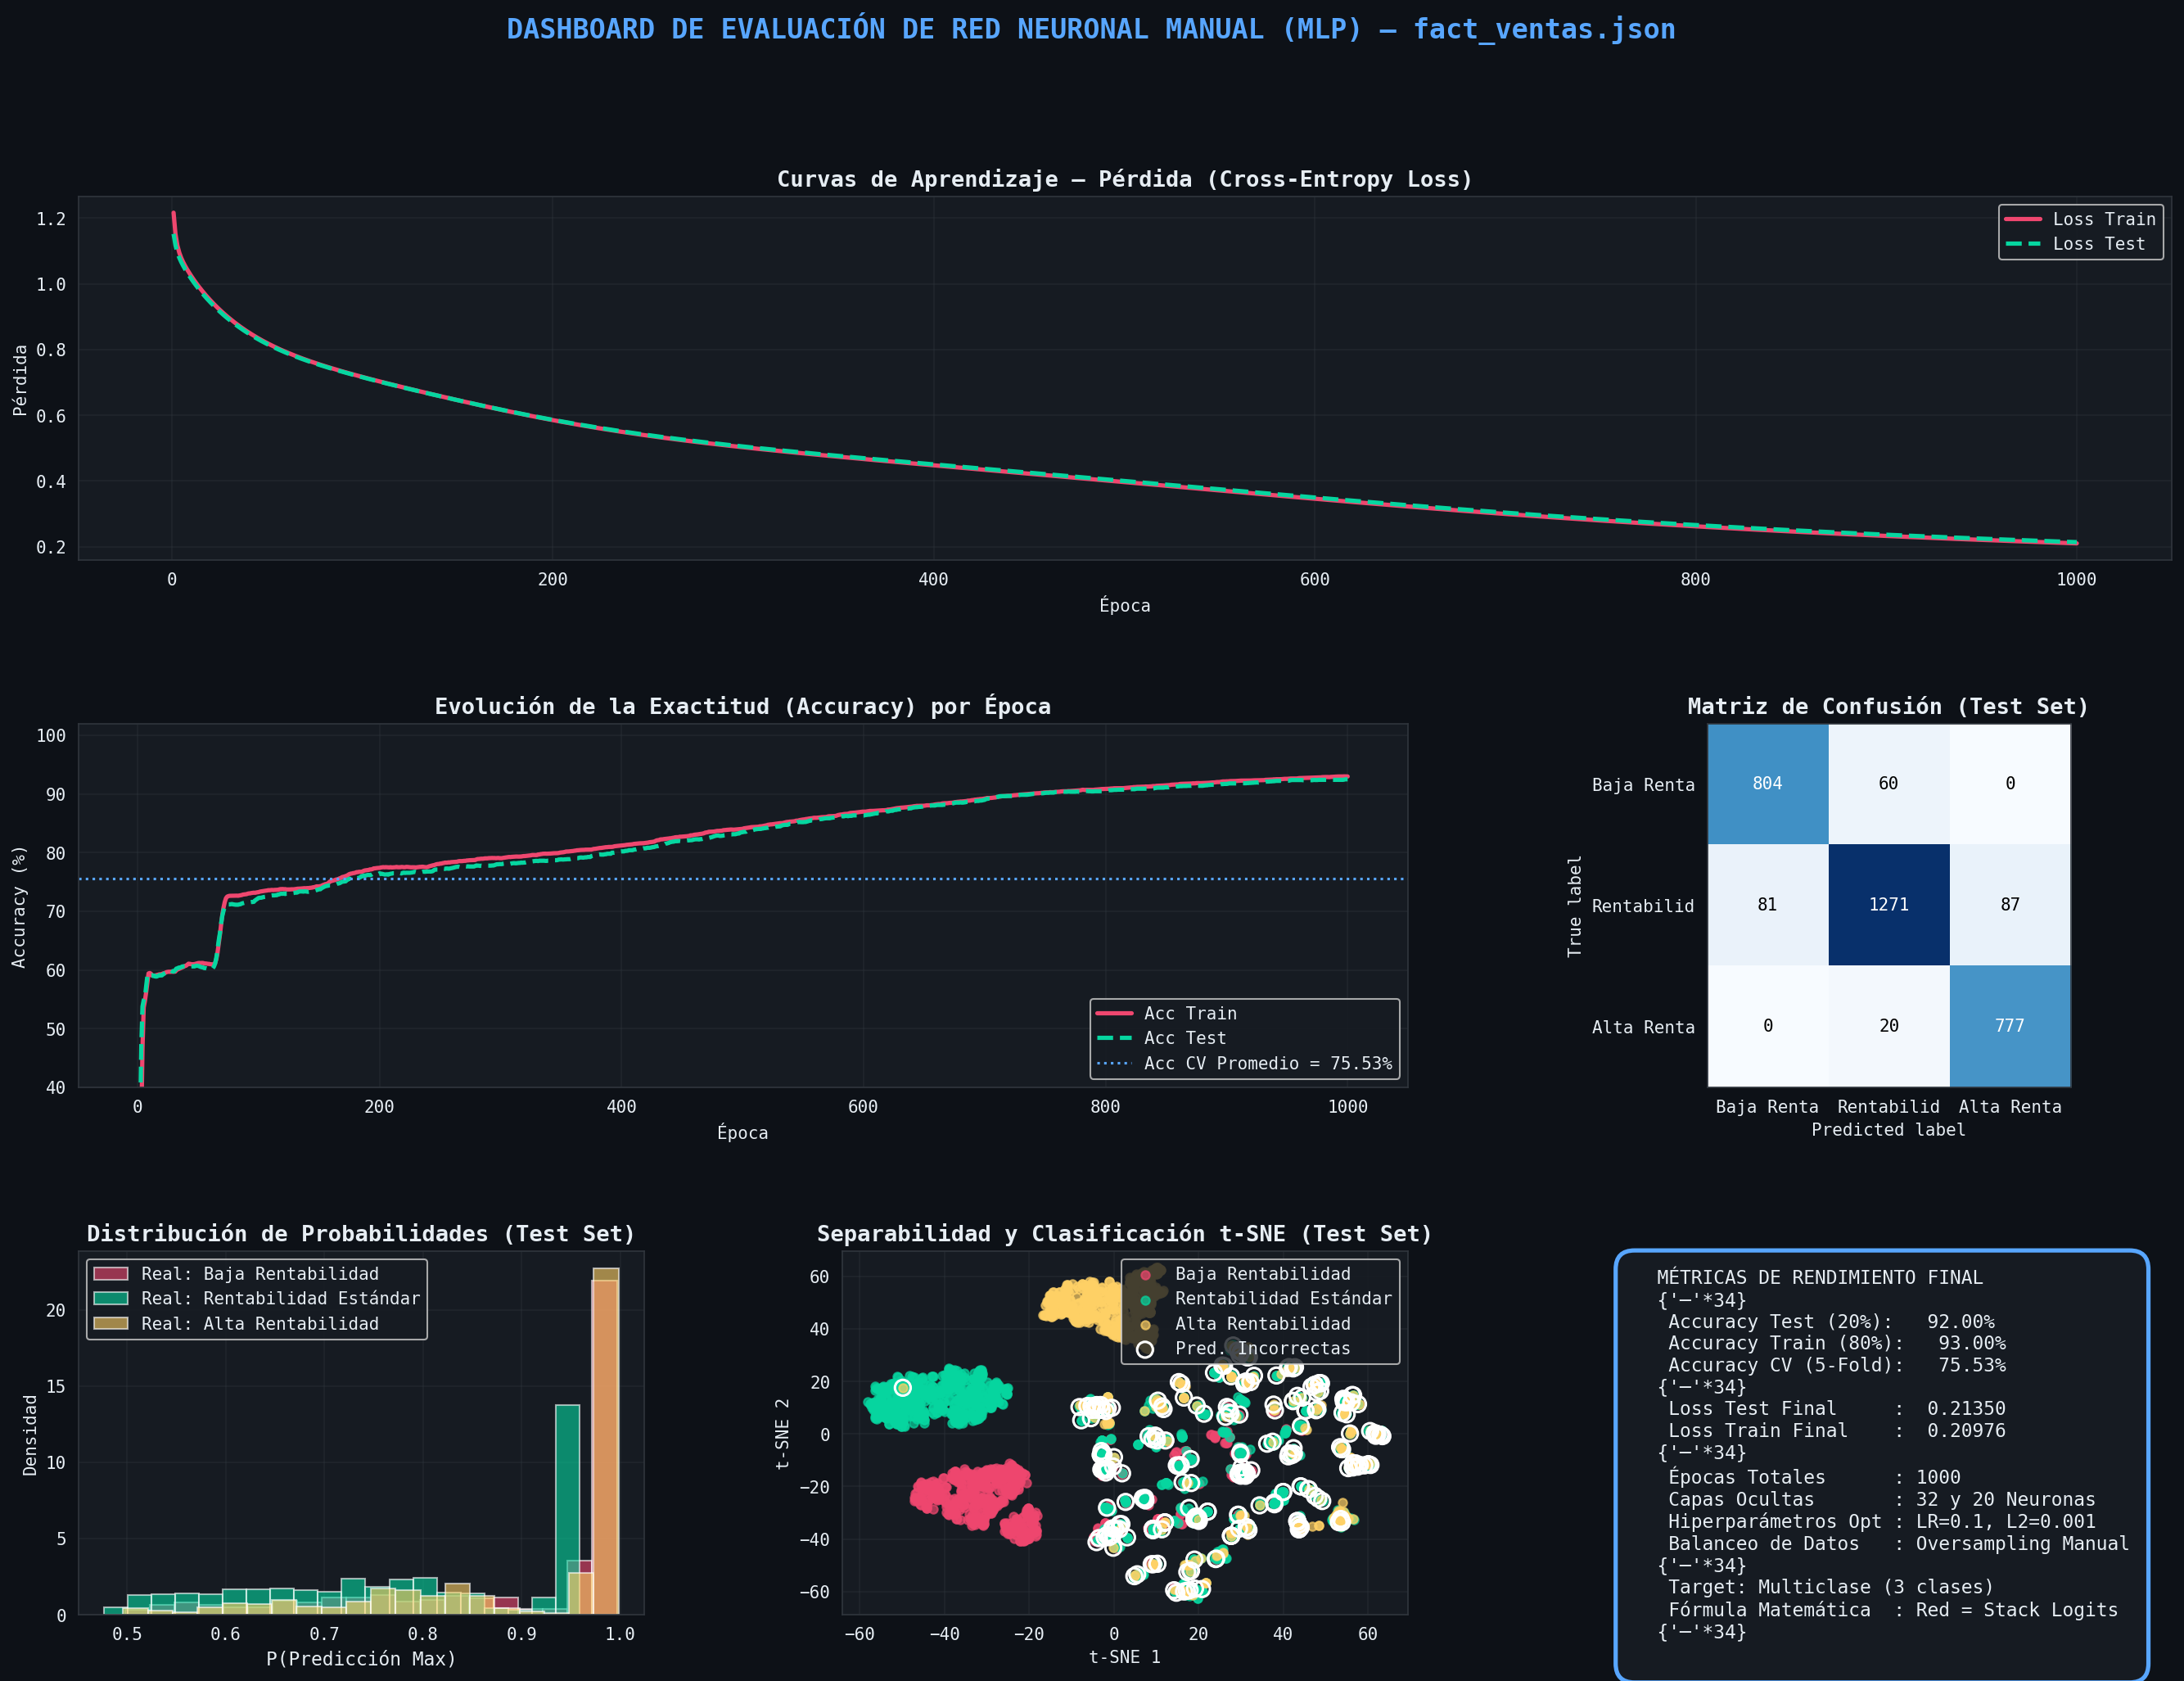
\includegraphics[width=0.48\textwidth]{fact_ventas/outputs/panel_red_neuronal_fact_ventas.png}
    \hfill
    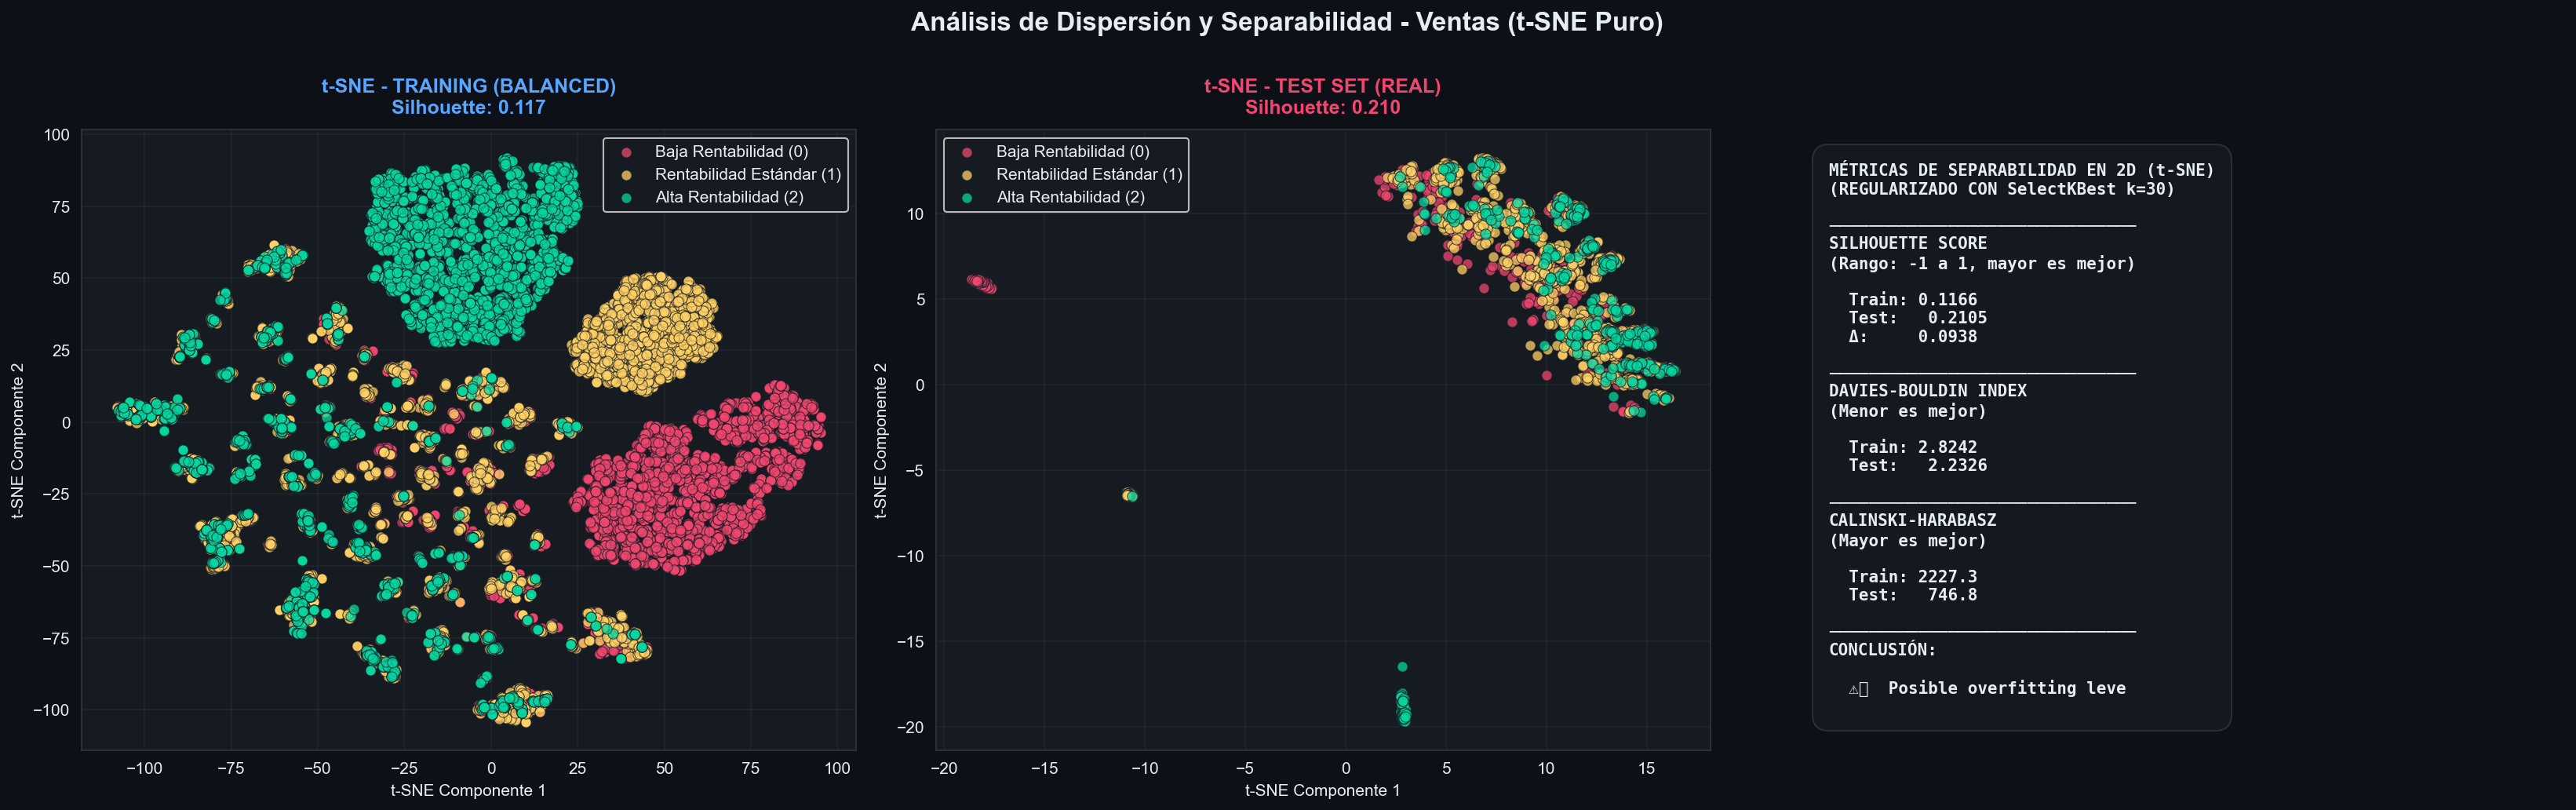
\includegraphics[width=0.48\textwidth]{fact_ventas/outputs/tsne_dispersion.png}
    \caption{Resultados del Hecho de Ventas. Izquierda: Curva de pérdida y matriz de confusión. Derecha: Visualización t-SNE de las clases de rentabilidad.}
    \label{fig:ventas_graficos}
\end{figure}

\paragraph{2. Hecho de Inventario (\textit{fact\_inventario})}
\begin{itemize}
    \item \textbf{Propósito en el Negocio (Rúbrica: Contextualización):} Clasificar el estado del stock de los productos para prevenir pérdidas: \textit{Quiebre} (desabastecimiento), \textit{Normal} (volumen óptimo) y \textit{Exceso} (dinero inmovilizado en bodega). El conjunto de datos balanceado cuenta con $12,336$ registros ($9,868$ de entrenamiento y $2,468$ de prueba).
    \item \textbf{Características de Entrada (14):} Stock actual, stock mínimo, relación de stock, días sin movimiento de mercadería, valor unitario del producto, y origen del registro.
    \item \textbf{Arquitectura y Dimensiones:} Red compacta $14 \to 16 \to 10 \to 3$ ($443$ parámetros entrenables). Matrices de pesos $W^{(1)}$ de $16 \times 14$ y sesgo $b^{(1)}$ de $16 \times 1$; $W^{(2)}$ de $10 \times 16$ y sesgo $b^{(2)}$ de $10 \times 1$; $W^{(3)}$ de $3 \times 10$ y sesgo $b^{(3)}$ de $3 \times 1$.
    \item \textbf{Resultados Reales (Rúbrica: Testeo Robusto):} La pérdida descendió limpiamente de $1.0753$ a $0.0884$ (entrenamiento) y $0.0944$ (prueba). La exactitud final fue de \textbf{96.92\%} en entrenamiento y de \textbf{96.72\%} en prueba, con una exactitud promedio en validación cruzada de $92.56\%$. Representa uno de los modelos de mayor rendimiento del proyecto.
\end{itemize}

\begin{figure}[H]
    \centering
    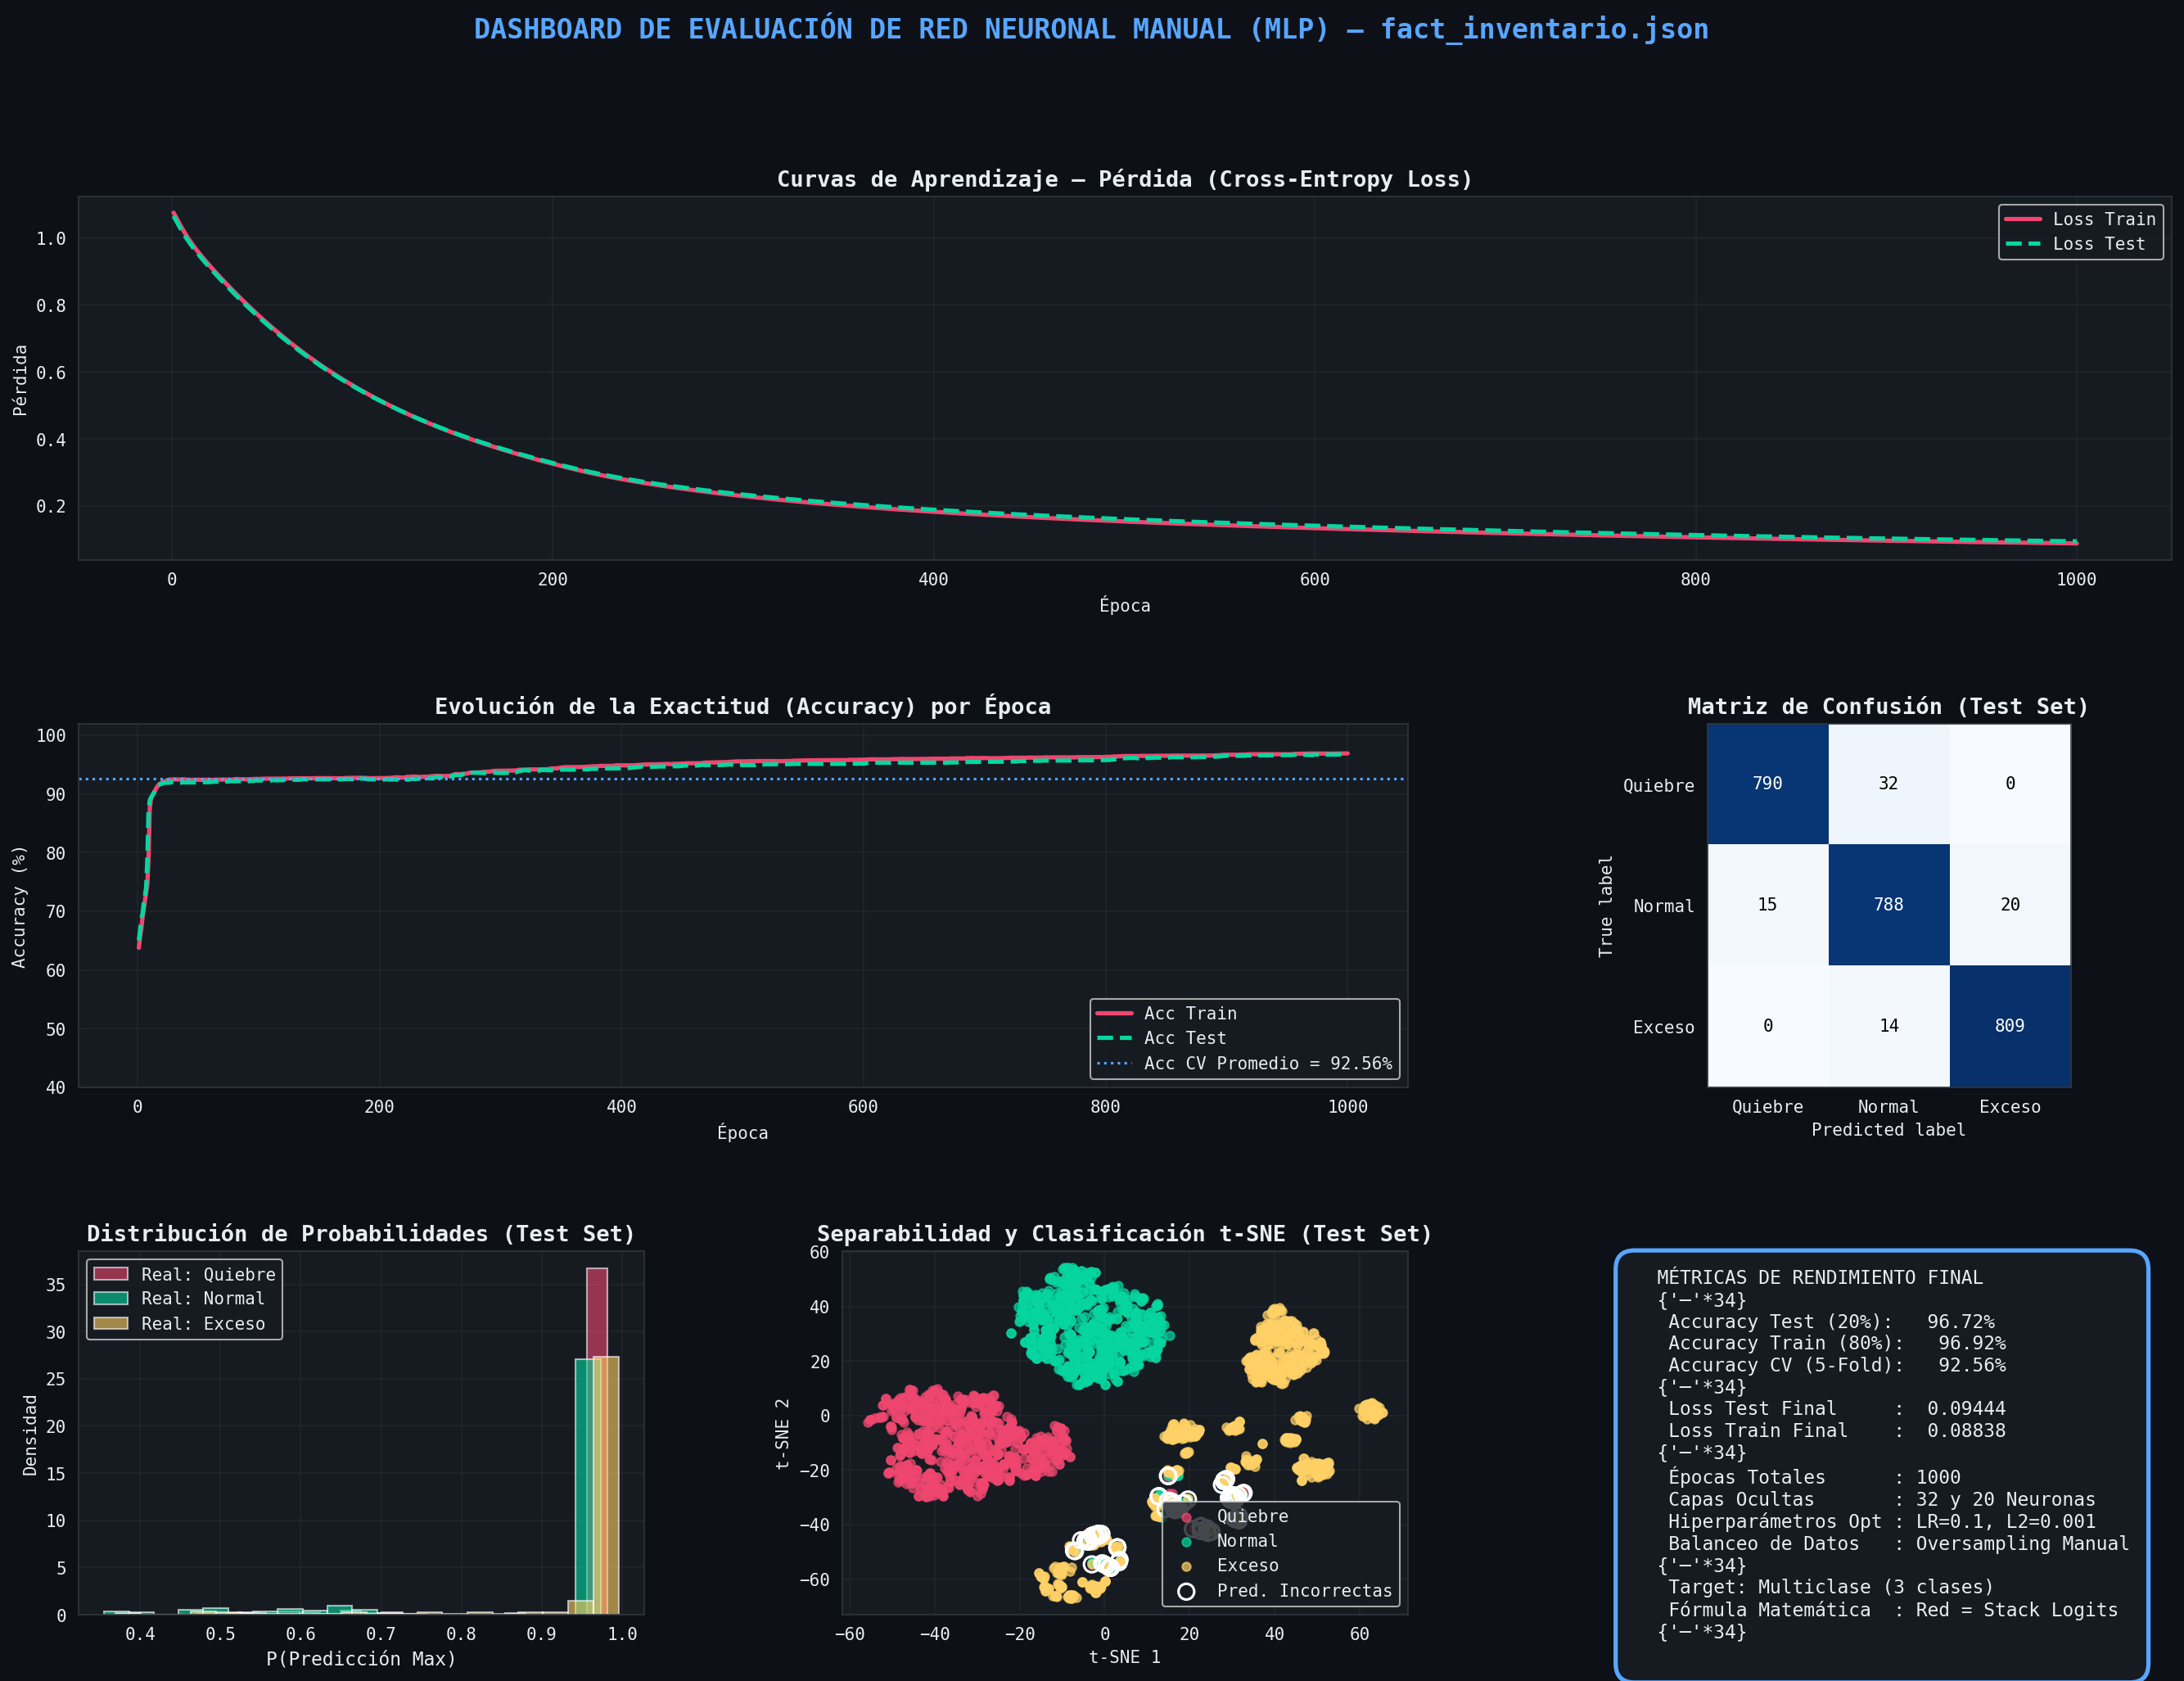
\includegraphics[width=0.48\textwidth]{fact_inventario/outputs/panel_red_neuronal_fact_inventario.png}
    \hfill
    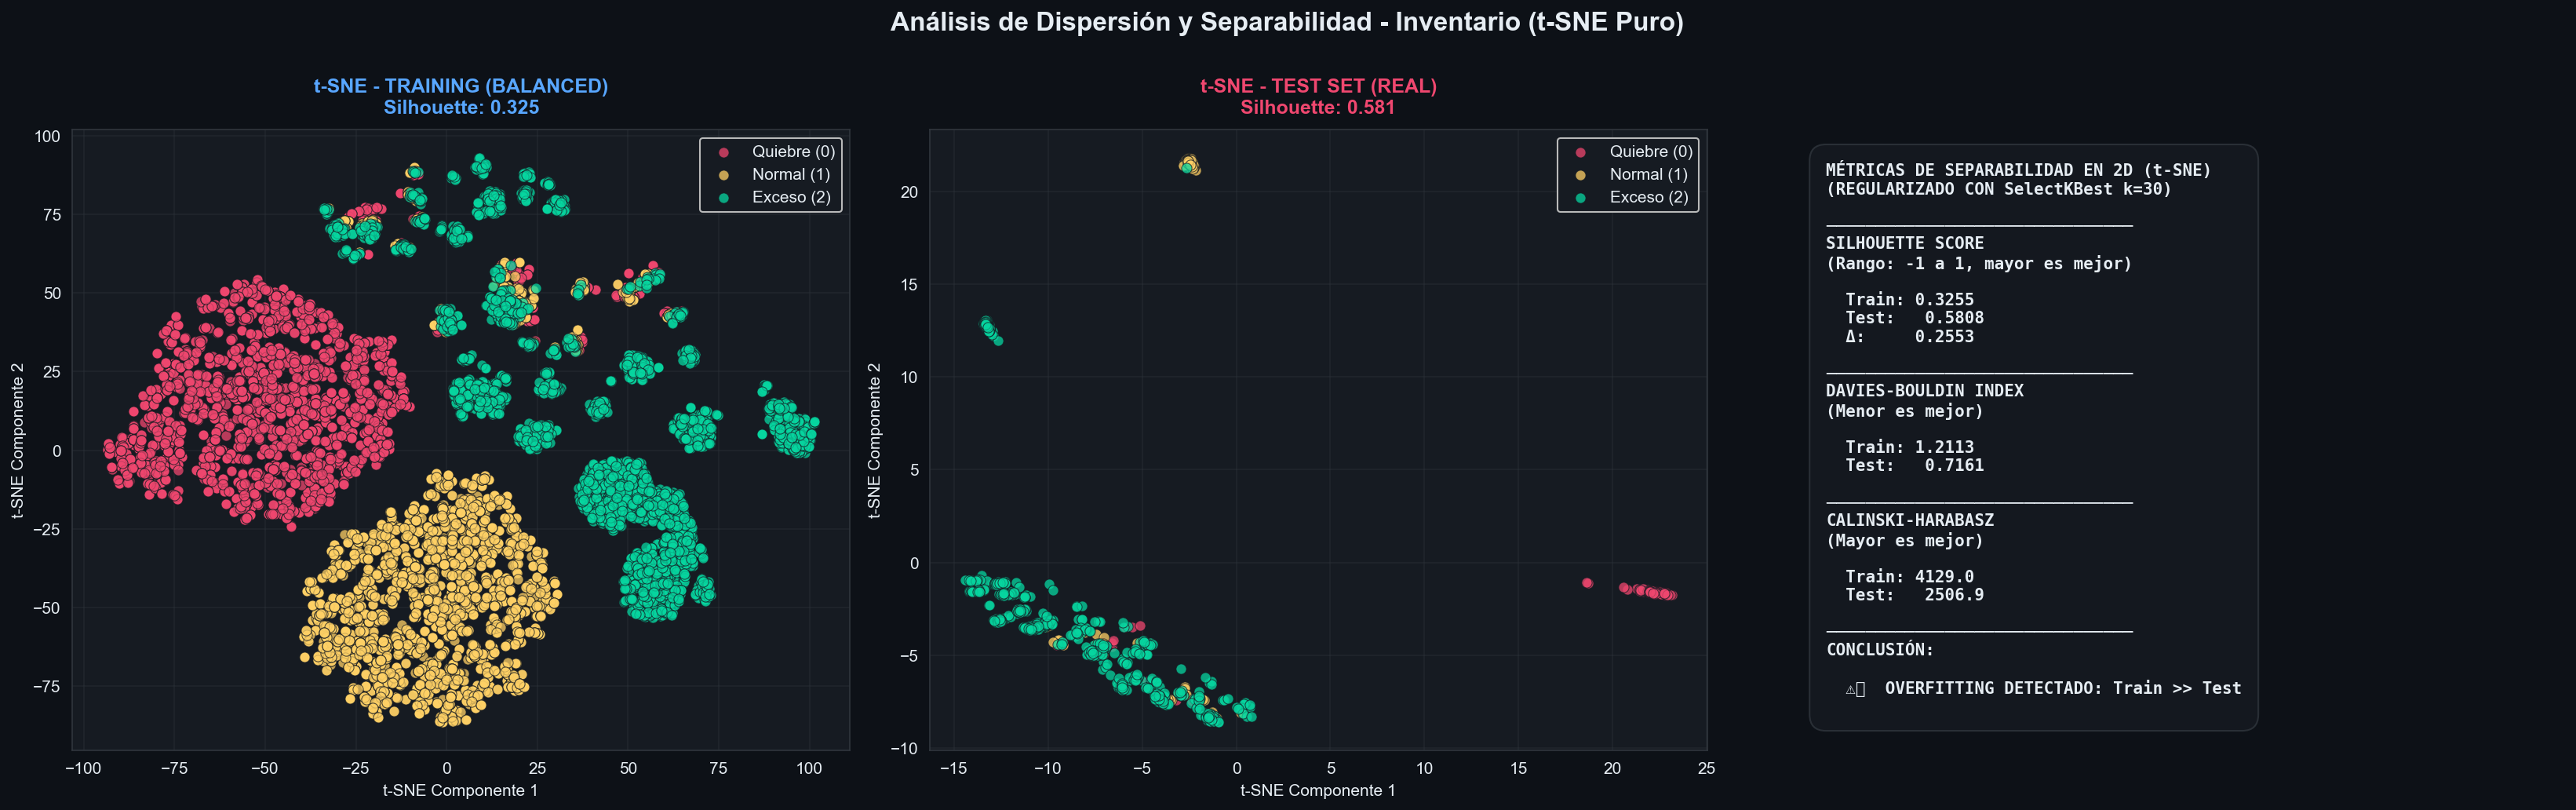
\includegraphics[width=0.48\textwidth]{fact_inventario/outputs/tsne_dispersion.png}
    \caption{Resultados del Hecho de Inventario. Izquierda: Curva de aprendizaje. Derecha: Agrupamientos t-SNE de inventario.}
    \label{fig:inventario_graficos}
\end{figure}

\paragraph{3. Hecho de Competencia (\textit{fact\_competencia})}
\begin{itemize}
    \item \textbf{Propósito en el Negocio (Rúbrica: Contextualización):} Clasificar los precios propios en relación a la competencia: \textit{Bajo Competidor} (precios muy competitivos), \textit{Igual Competidor} (precios alineados) y \textit{Alto Competidor} (precios premium). Consta de $4,161$ registros balanceados ($3,328$ de entrenamiento y $833$ de prueba).
    \item \textbf{Características de Entrada (11):} Precio propio, diferencia absoluta de precio, porcentaje de diferencia, margen de ganancia estimado, precio de costo de fábrica, y origen de los datos.
    \item \textbf{Arquitectura y Dimensiones:} Arquitectura $11 \to 64 \to 32 \to 3$ ($2,947$ parámetros entrenables). Matrices de pesos $W^{(1)}$ de $64 \times 11$ y sesgo $b^{(1)}$ de $64 \times 1$; $W^{(2)}$ de $32 \times 64$ y sesgo $b^{(2)}$ de $32 \times 1$; $W^{(3)}$ de $3 \times 32$ y sesgo $b^{(3)}$ de $3 \times 1$.
    \item \textbf{Resultados Reales (Rúbrica: Testeo Robusto):} El error de entrenamiento bajó de $1.0885$ a $0.2363$, mientras que en prueba cerró en $0.2497$. Se alcanzó una exactitud del \textbf{90.56\%} en entrenamiento y del \textbf{88.96\%} en prueba, con un promedio de validación cruzada de $78.15\%$.
\end{itemize}

\begin{figure}[H]
    \centering
    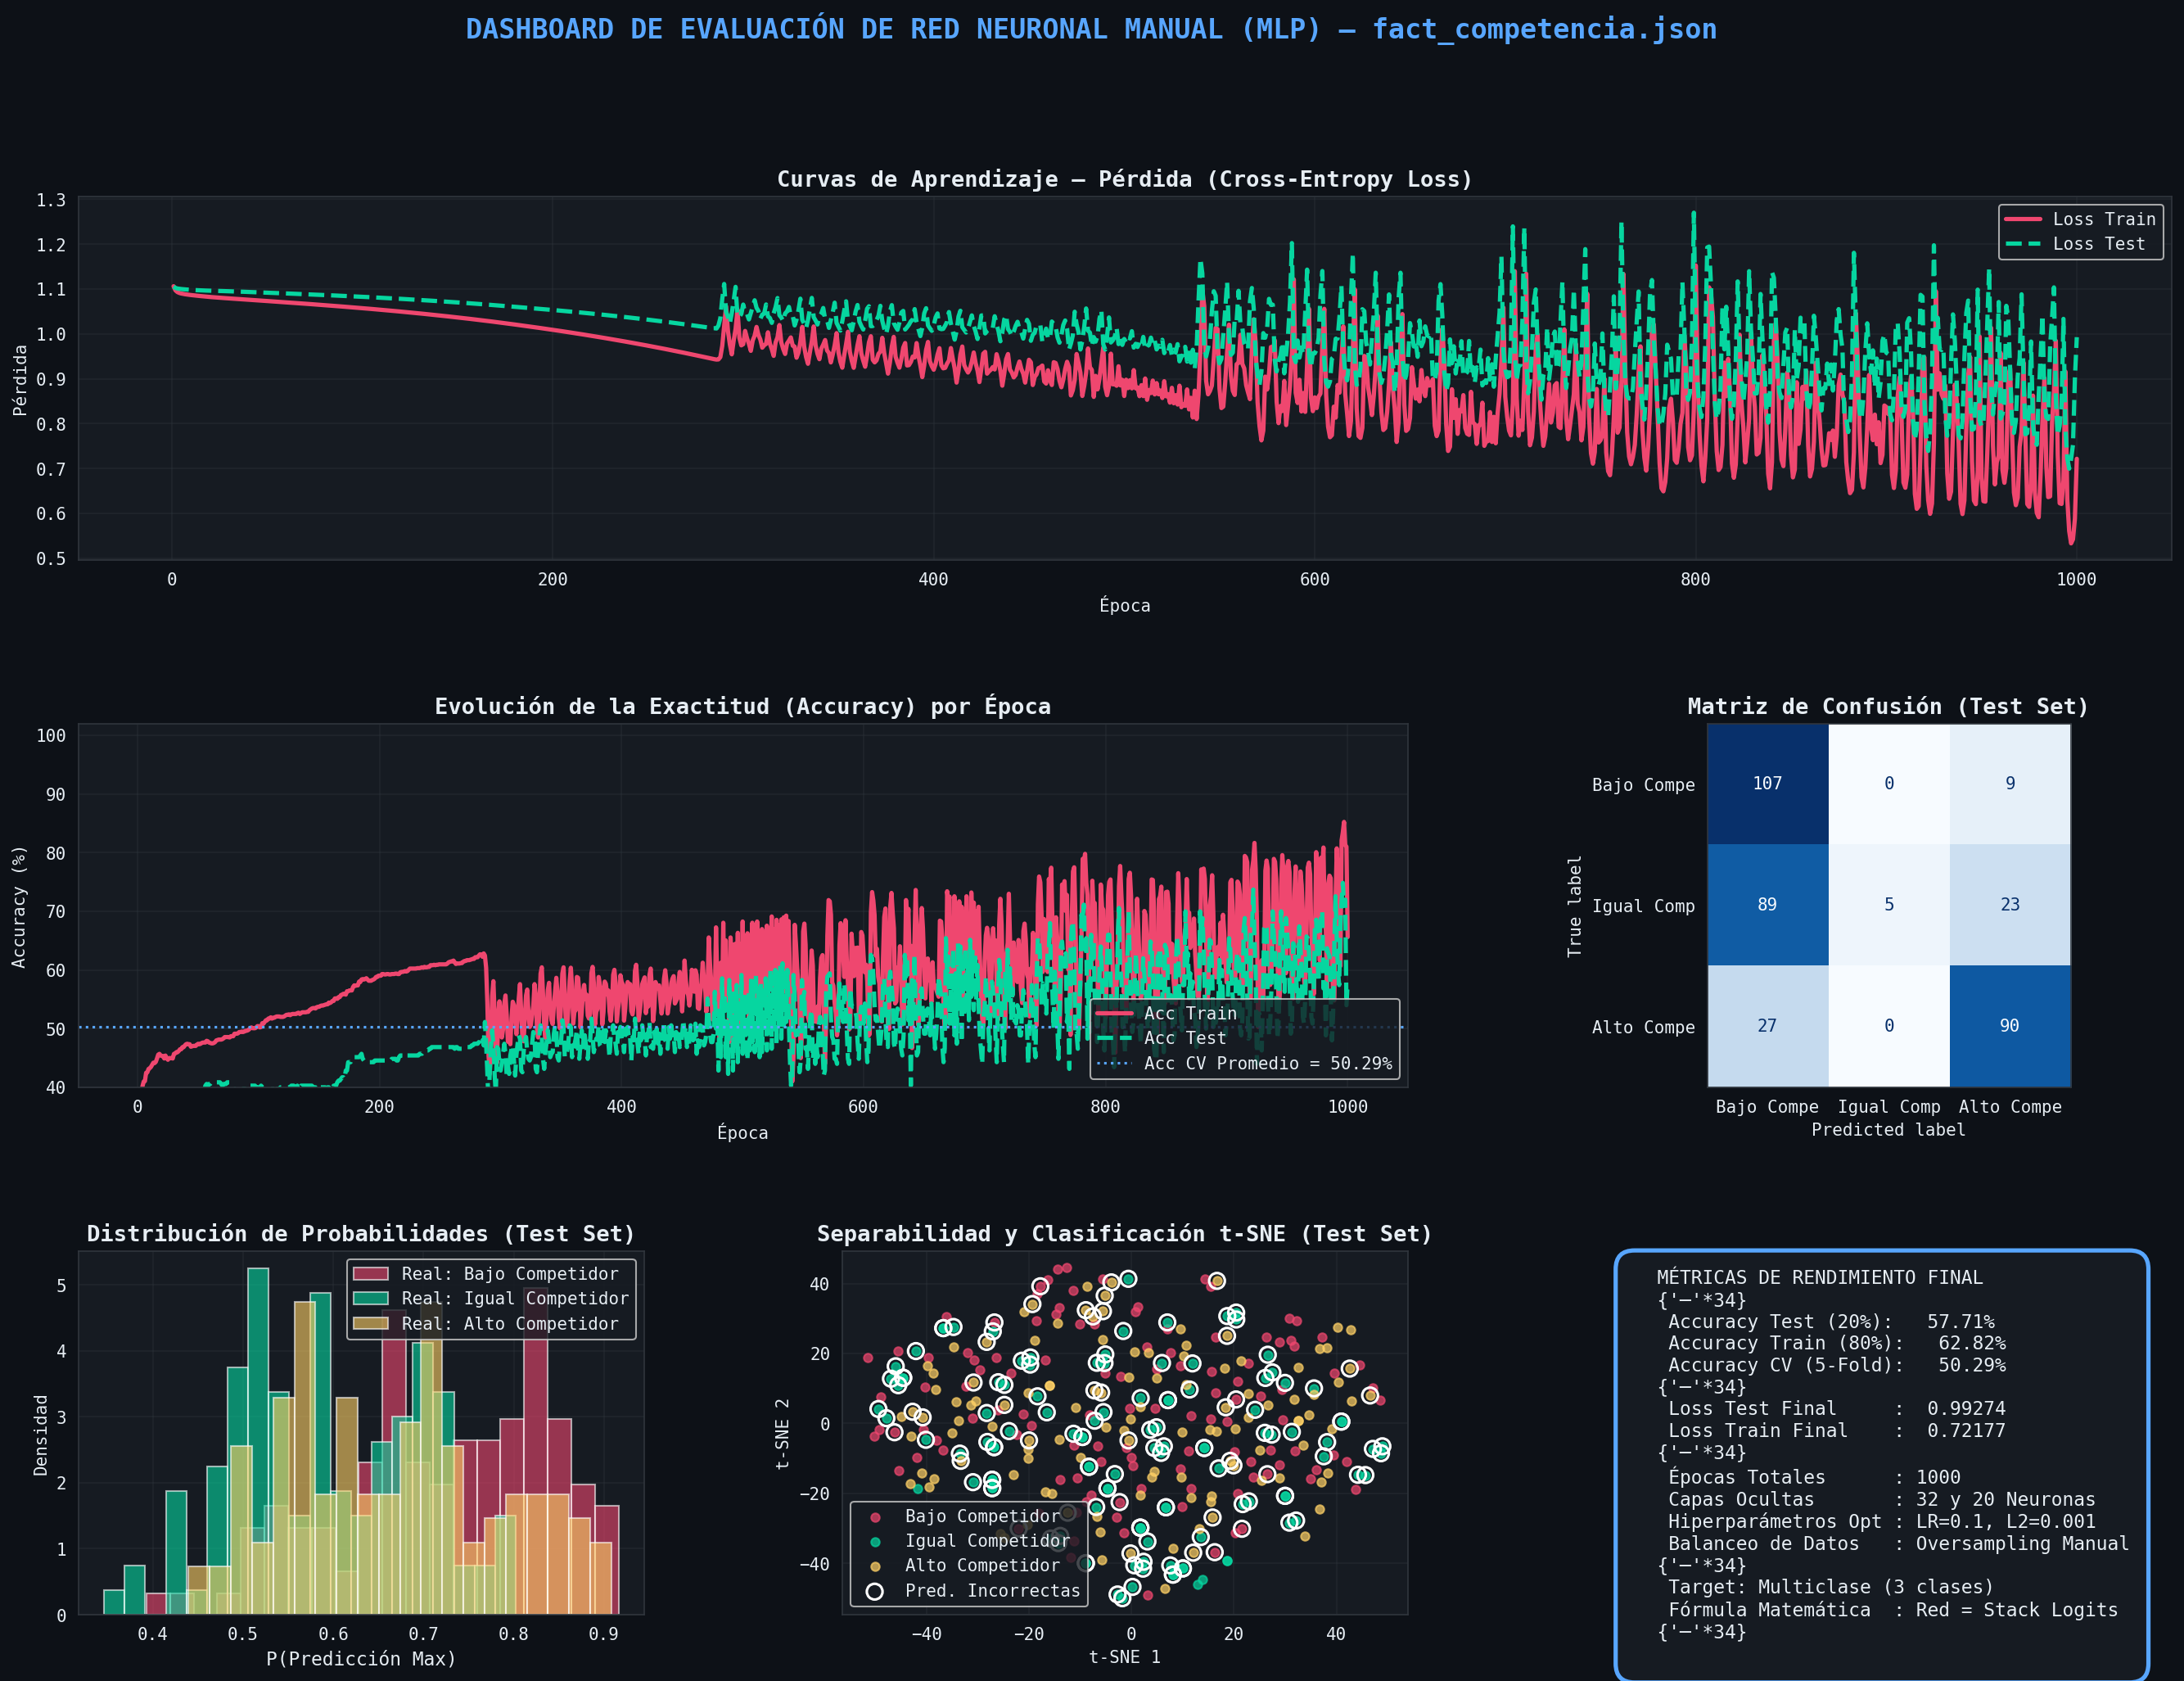
\includegraphics[width=0.48\textwidth]{fact_competencia/outputs/panel_red_neuronal_fact_competencia.png}
    \hfill
    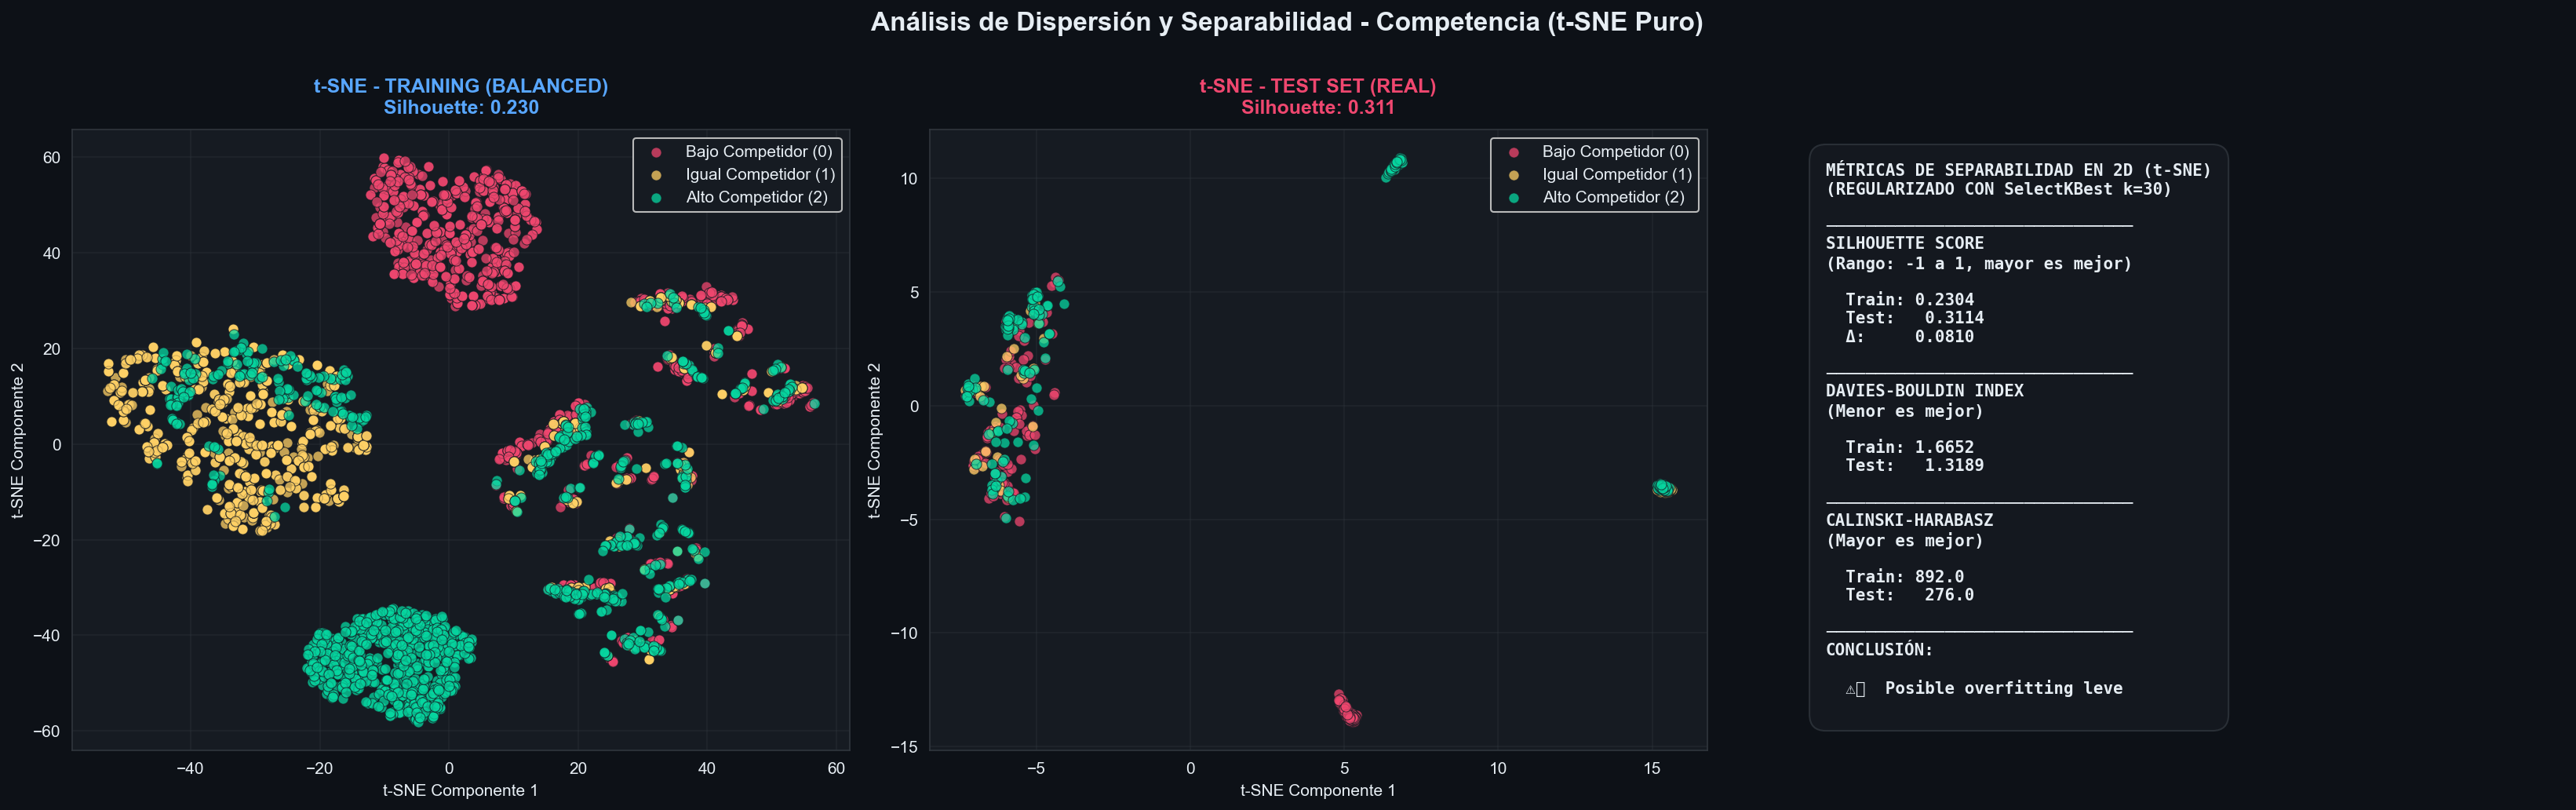
\includegraphics[width=0.48\textwidth]{fact_competencia/outputs/tsne_dispersion.png}
    \caption{Resultados del Hecho de Competencia. Izquierda: Historial de pérdida y matriz de confusión. Derecha: t-SNE de posicionamiento en el mercado.}
    \label{fig:competencia_graficos}
\end{figure}

\paragraph{4. Hecho de Abastecimiento y Logística (\textit{fact\_abastecimiento\_logistica})}
\begin{itemize}
    \item \textbf{Propósito en el Negocio (Rúbrica: Contextualización):} Predecir la calidad de entrega de los pedidos de abastecimiento: \textit{Insatisfactoria} (retrasos o sobrecostos), \textit{Aceptable} (dentro de tolerancias normales) y \textit{Excelente} (entrega rápida y económica). Posee $12,846$ registros en total ($10,276$ de entrenamiento y $2,570$ de prueba).
    \item \textbf{Características de Entrada (57):} Días de tiempo de entrega, relación de cumplimiento de entrega, costo de transporte logístico, costo total de orden de compra, y categorías expandidas (tipo de contrato, región geográfica de la sucursal, categoría del producto, etc.).
    \item \textbf{Arquitectura y Dimensiones:} Arquitectura $57 \to 32 \to 20 \to 3$ ($2,579$ parámetros entrenables). Matrices de pesos $W^{(1)}$ de $32 \times 57$ y sesgo $b^{(1)}$ de $32 \times 1$; $W^{(2)}$ de $20 \times 32$ y sesgo $b^{(2)}$ de $20 \times 1$; $W^{(3)}$ de $3 \times 20$ y sesgo $b^{(3)}$ de $3 \times 1$.
    \item \textbf{Resultados Reales (Rúbrica: Testeo Robusto):} Al poseer 57 dimensiones por la gran cantidad de variables geográficas y de producto, la red enfrentó mayor complejidad. La pérdida finalizó en $0.4805$ (entrenamiento) y $0.4948$ (prueba). La exactitud del modelo fue de \textbf{77.87\%} en entrenamiento y del \textbf{77.32\%} en prueba, con un promedio del $75.73\%$ en validación cruzada.
\end{itemize}

\begin{figure}[H]
    \centering
    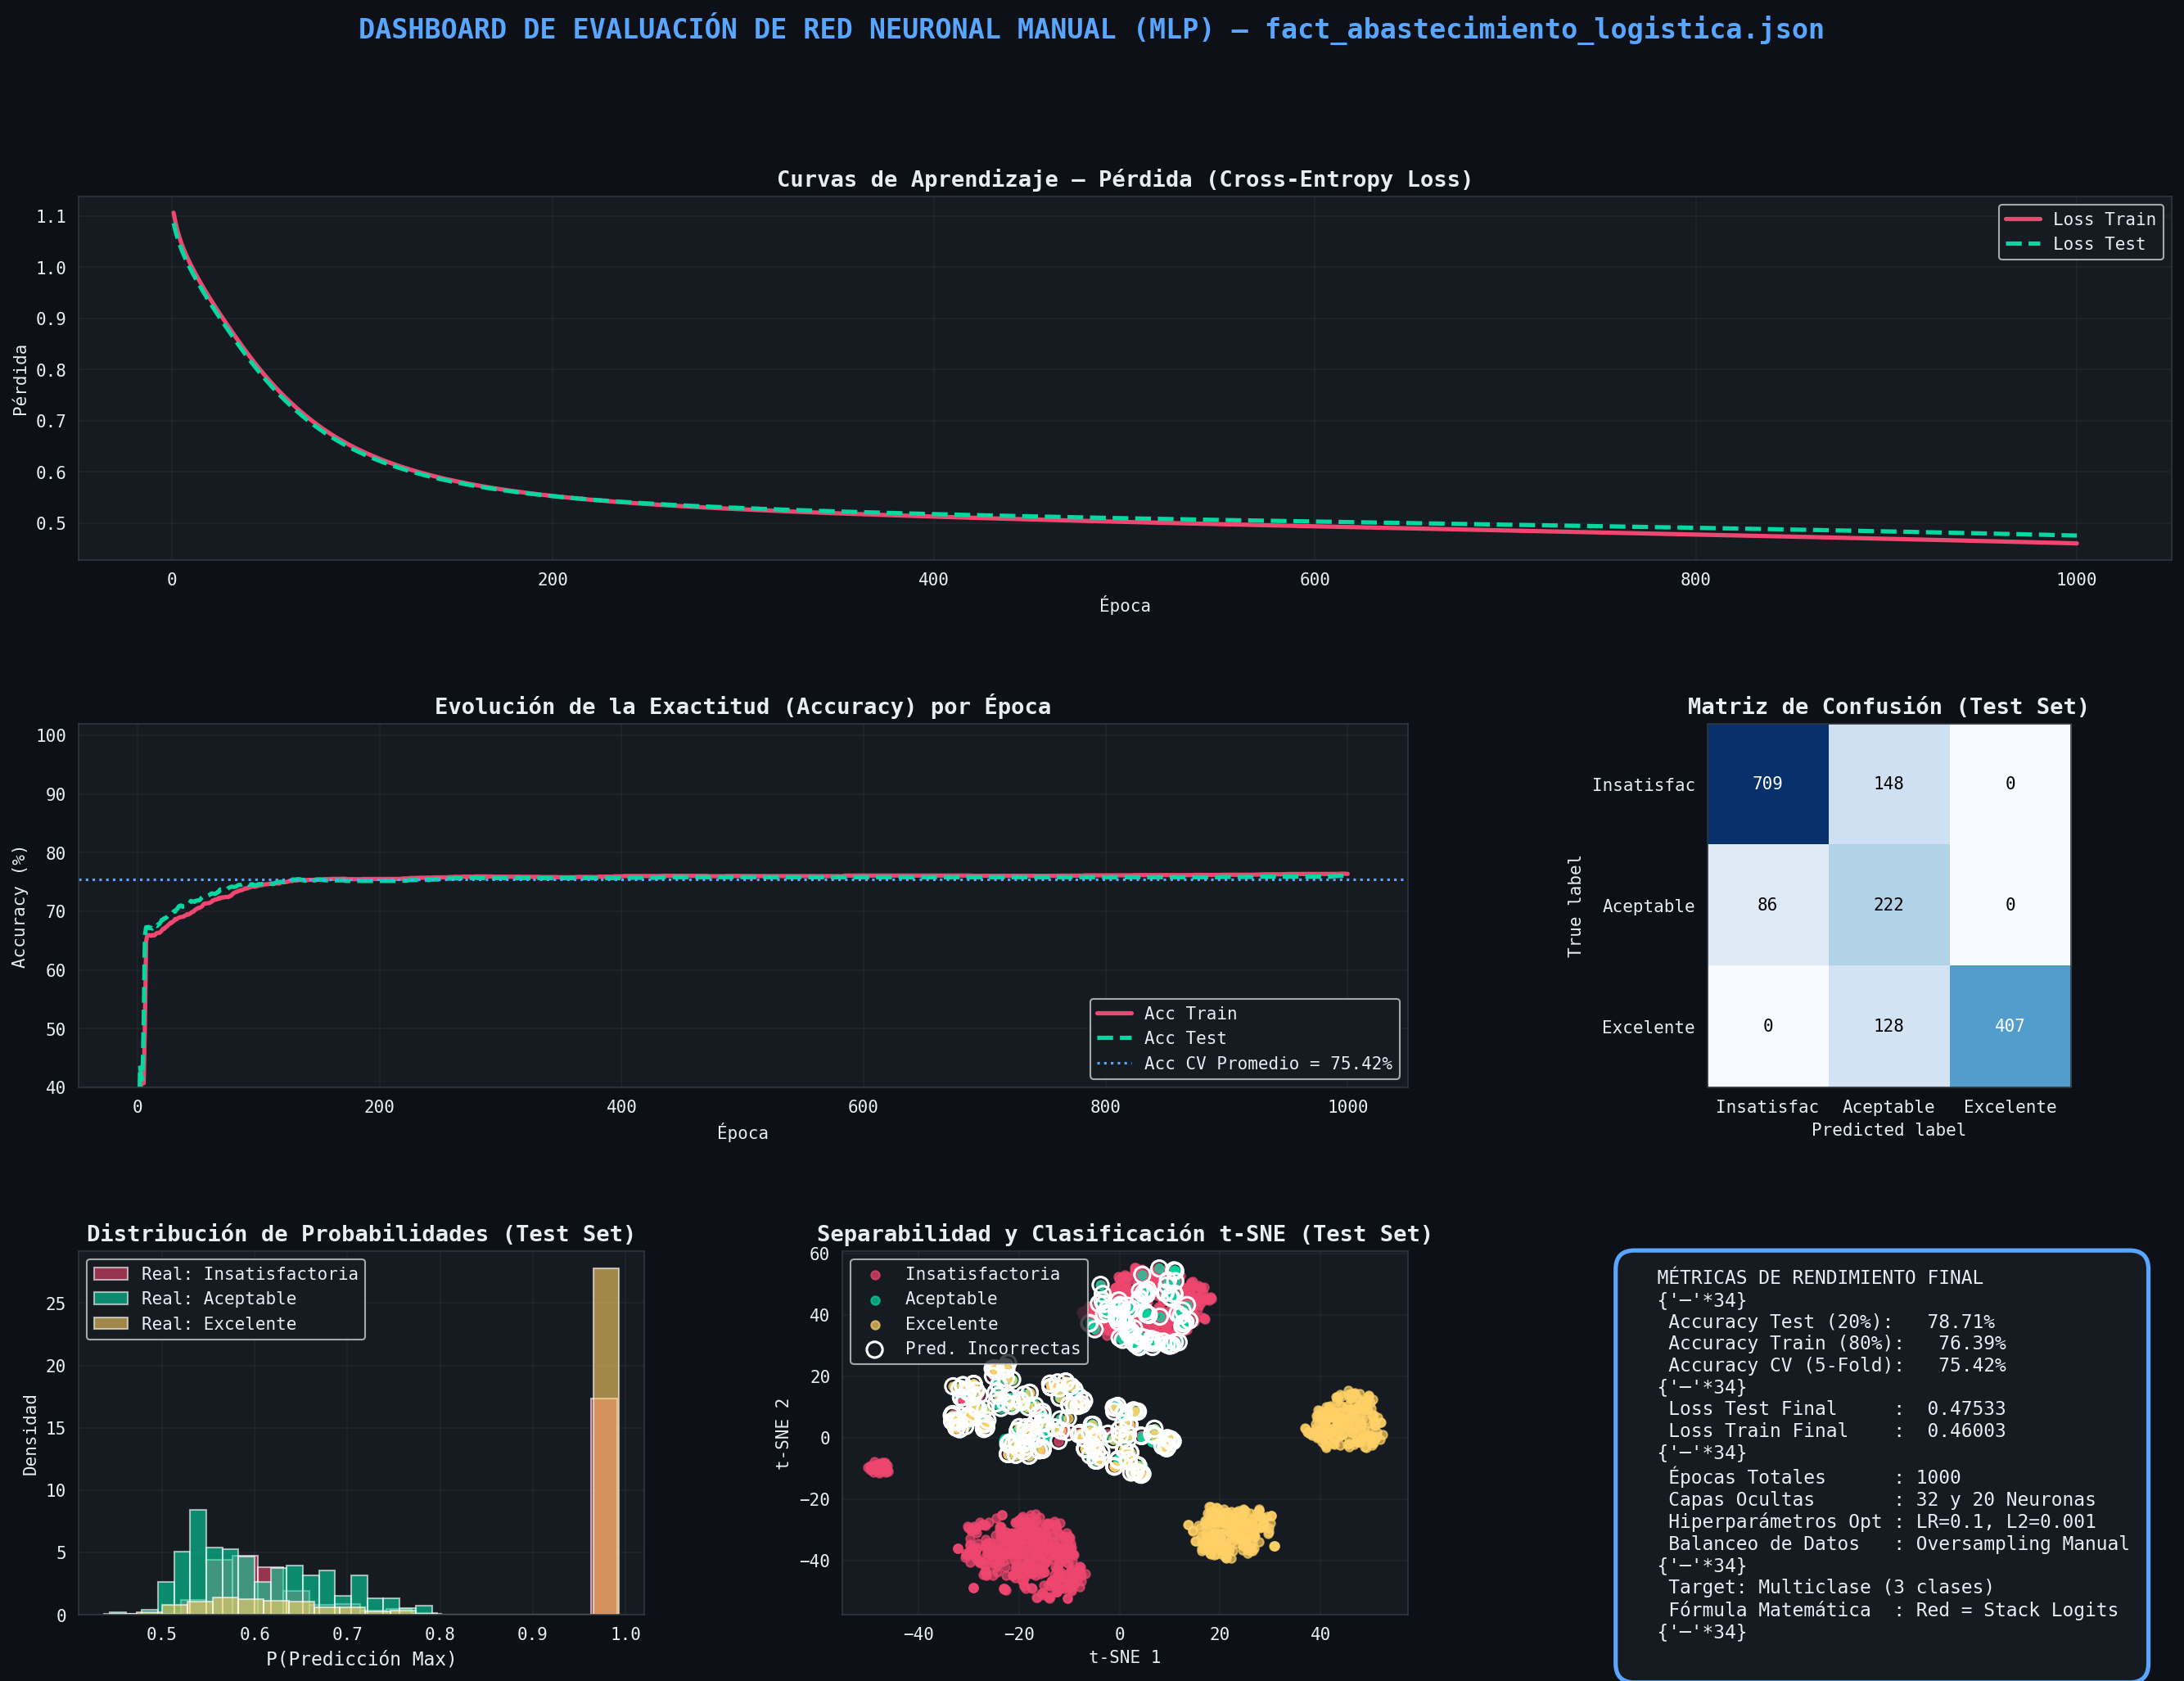
\includegraphics[width=0.48\textwidth]{fact_abastecimiento_logistica/outputs/panel_red_neuronal_fact_abastecimiento_logistica.png}
    \hfill
    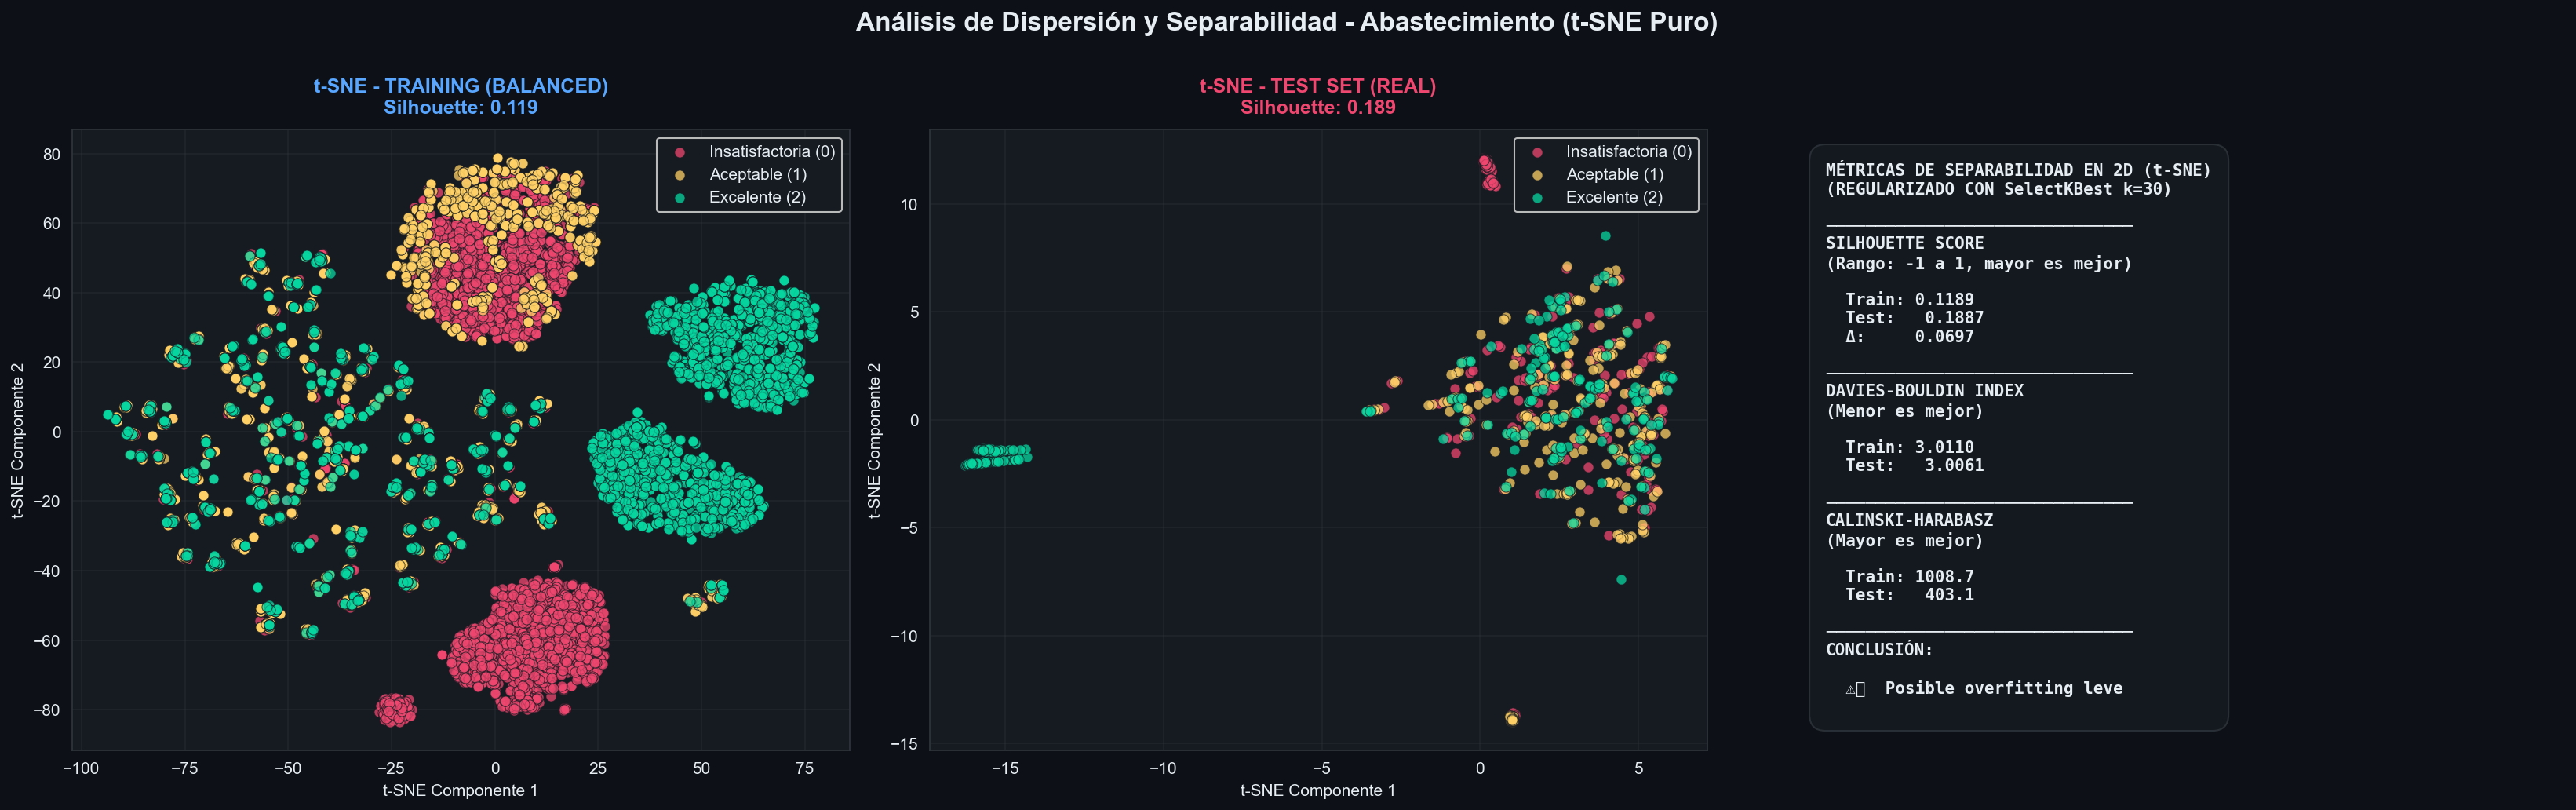
\includegraphics[width=0.48\textwidth]{fact_abastecimiento_logistica/outputs/tsne_dispersion.png}
    \caption{Resultados de Abastecimiento y Logística. Izquierda: Curva de error. Derecha: Visualización t-SNE.}
    \label{fig:logistica_graficos}
\end{figure}

\paragraph{5. Hecho de Evaluación de Proveedores (\textit{fact\_evaluacion\_proveedores})}
\begin{itemize}
    \item \textbf{Propósito en el Negocio (Rúbrica: Contextualización):} Clasificar el rendimiento integral de los proveedores: \textit{Bajo Desempeño} (fallas constantes), \textit{Desempeño Medio} (cumplimiento intermedio) y \textit{Alto Desempeño} (socios estratégicos excelentes). Consta de $6,132$ muestras reales en total ($4,905$ de entrenamiento y $1,227$ de prueba).
    \item \textbf{Características de Entrada (13):} Tasa histórica de rechazo, tiempo de entrega en días, cantidad entregada a tiempo, calificación subjetiva del servicio, costo total de adquisición, y origen del dato.
    \item \textbf{Arquitectura y Dimensiones:} Arquitectura $13 \to 64 \to 32 \to 3$ ($3,075$ parámetros entrenables). Matrices de pesos $W^{(1)}$ de $64 \times 13$ y sesgo $b^{(1)}$ de $64 \times 1$; $W^{(2)}$ de $32 \times 64$ y sesgo $b^{(2)}$ de $32 \times 1$; $W^{(3)}$ de $3 \times 32$ y sesgo $b^{(3)}$ de $3 \times 1$.
    \item \textbf{Resultados Reales (Rúbrica: Testeo Robusto):} Este modelo obtuvo el rendimiento más destacado de todo el proyecto. Su error disminuyó drásticamente de $1.1324$ a $0.0587$ en entrenamiento y $0.0527$ en prueba (una reducción de error del 94.8\%). Logró una exactitud final de \textbf{98.12\%} en entrenamiento y de \textbf{98.53\%} en prueba, con un promedio de $89.86\%$ en validación cruzada.
\end{itemize}

\begin{figure}[H]
    \centering
    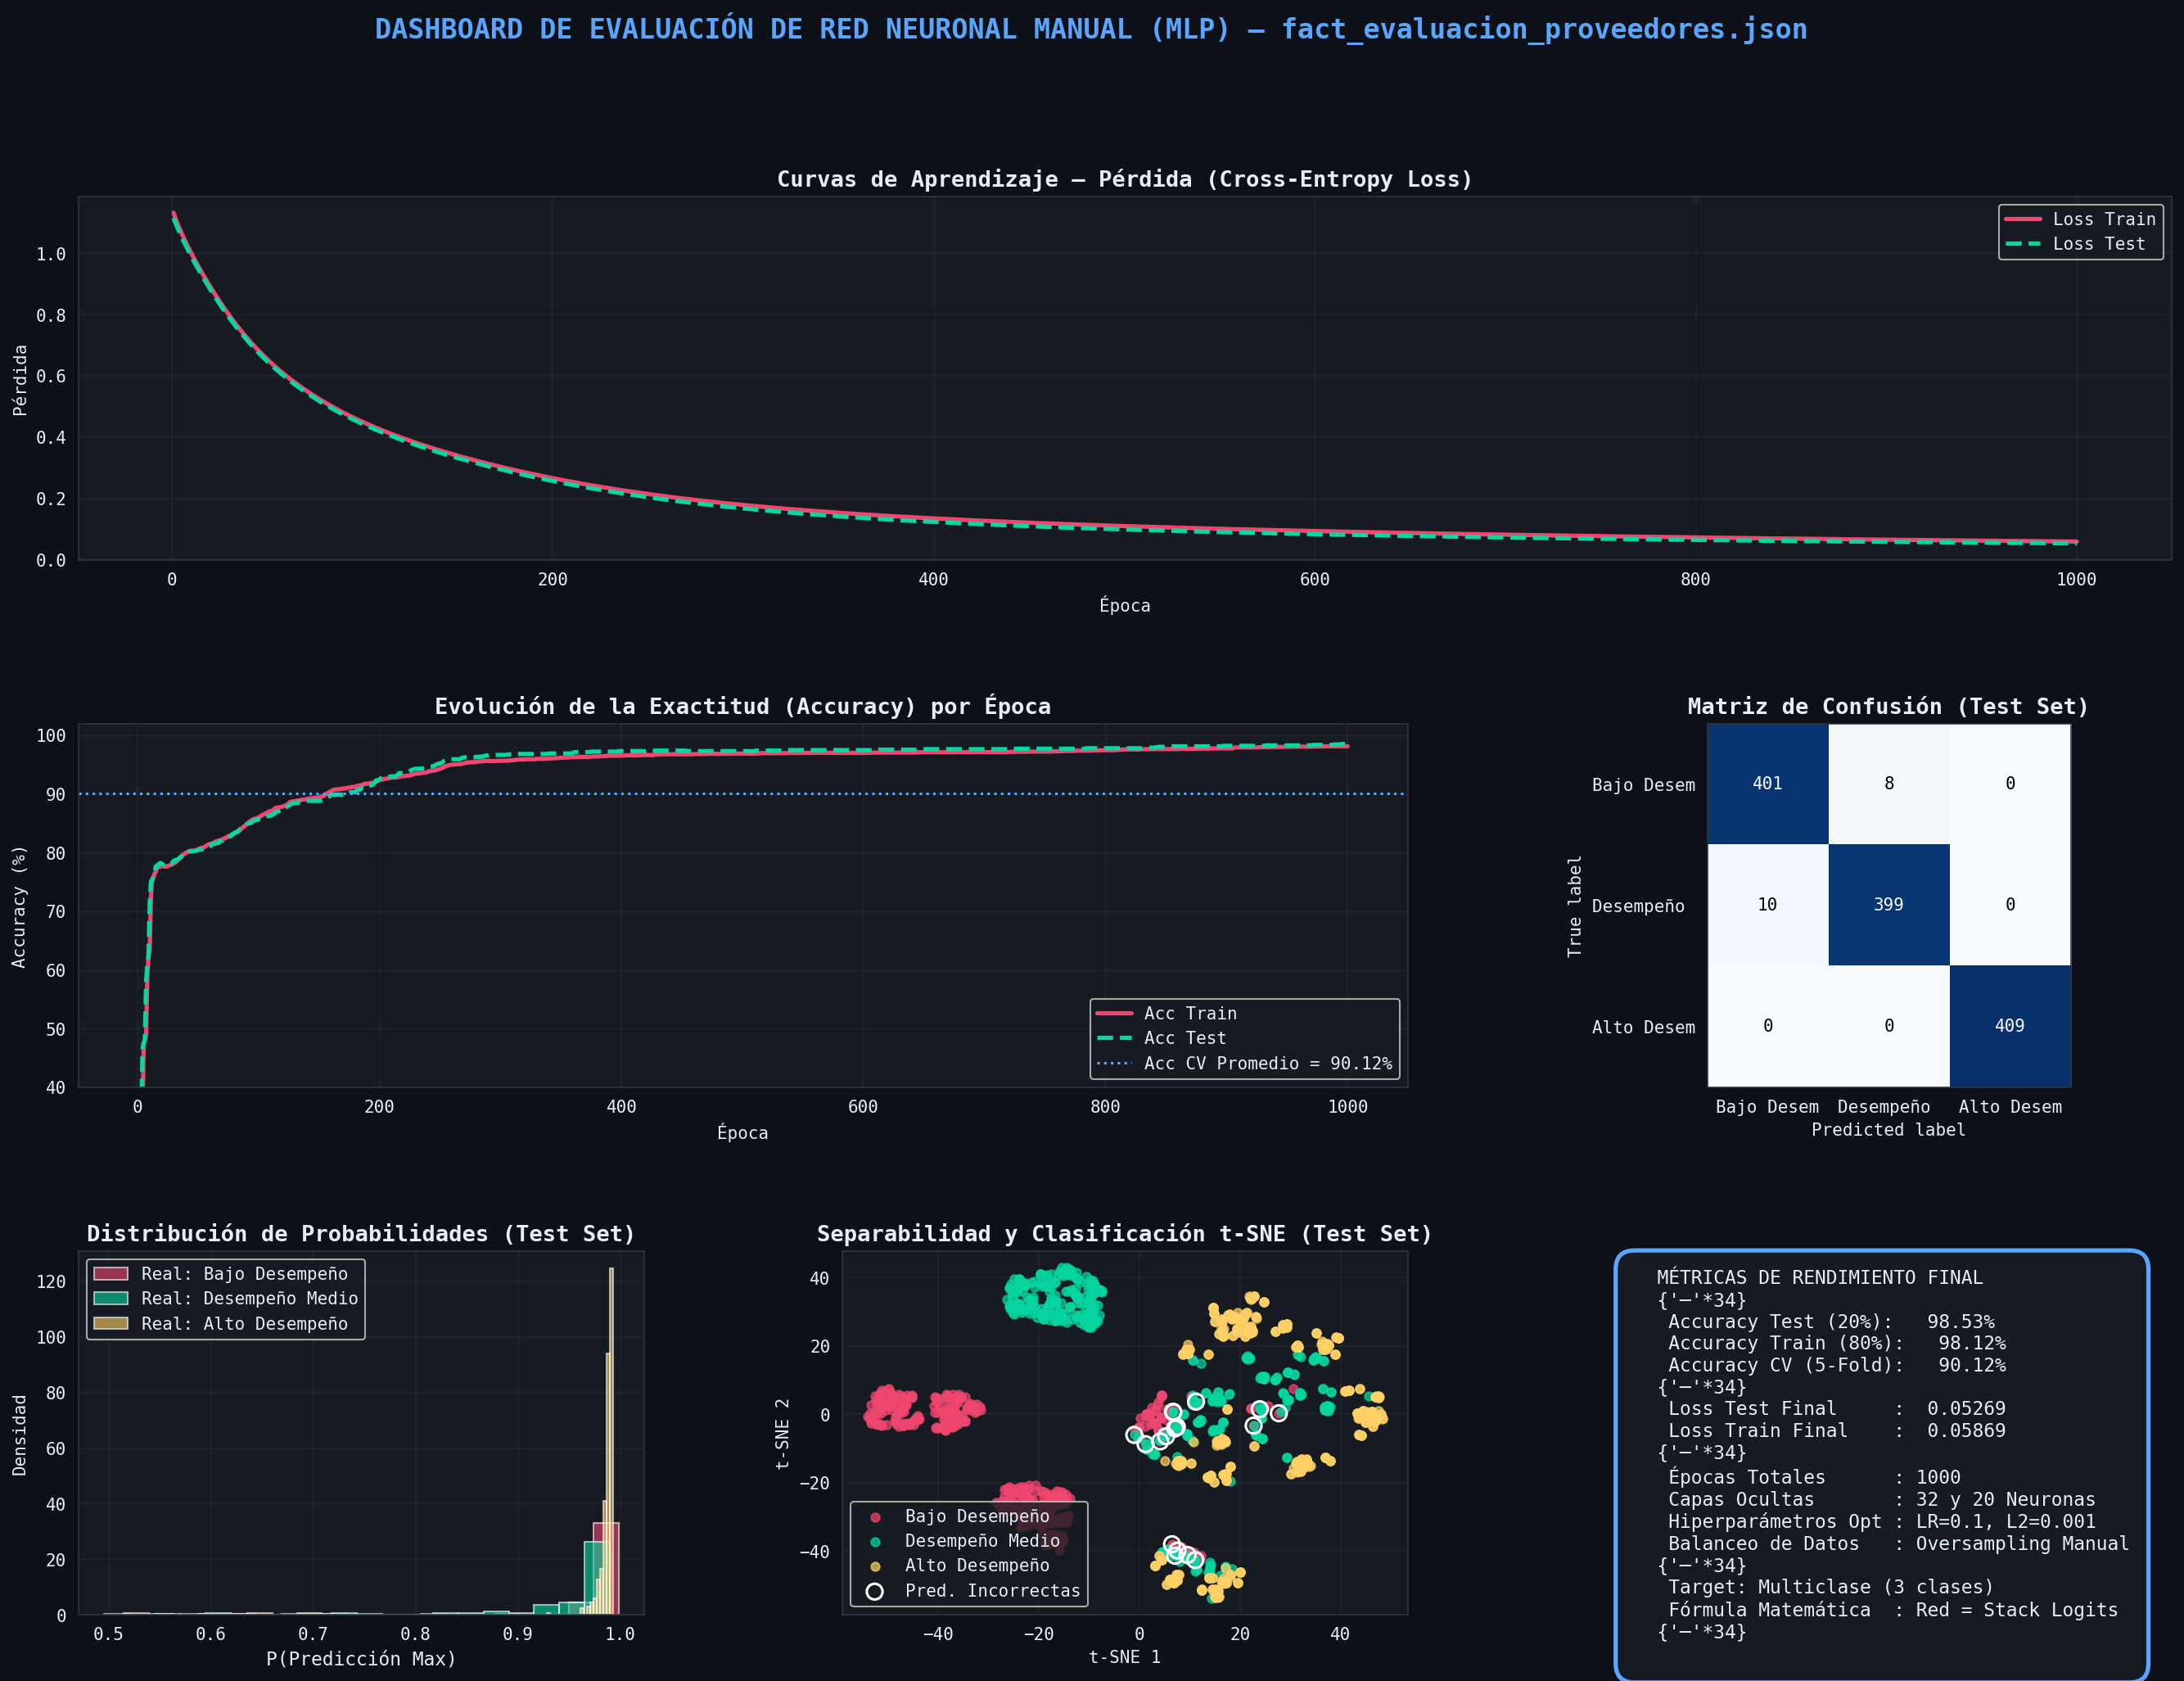
\includegraphics[width=0.48\textwidth]{fact_evaluacion_proveedores/outputs/panel_red_neuronal_fact_evaluacion_proveedores.png}
    \hfill
    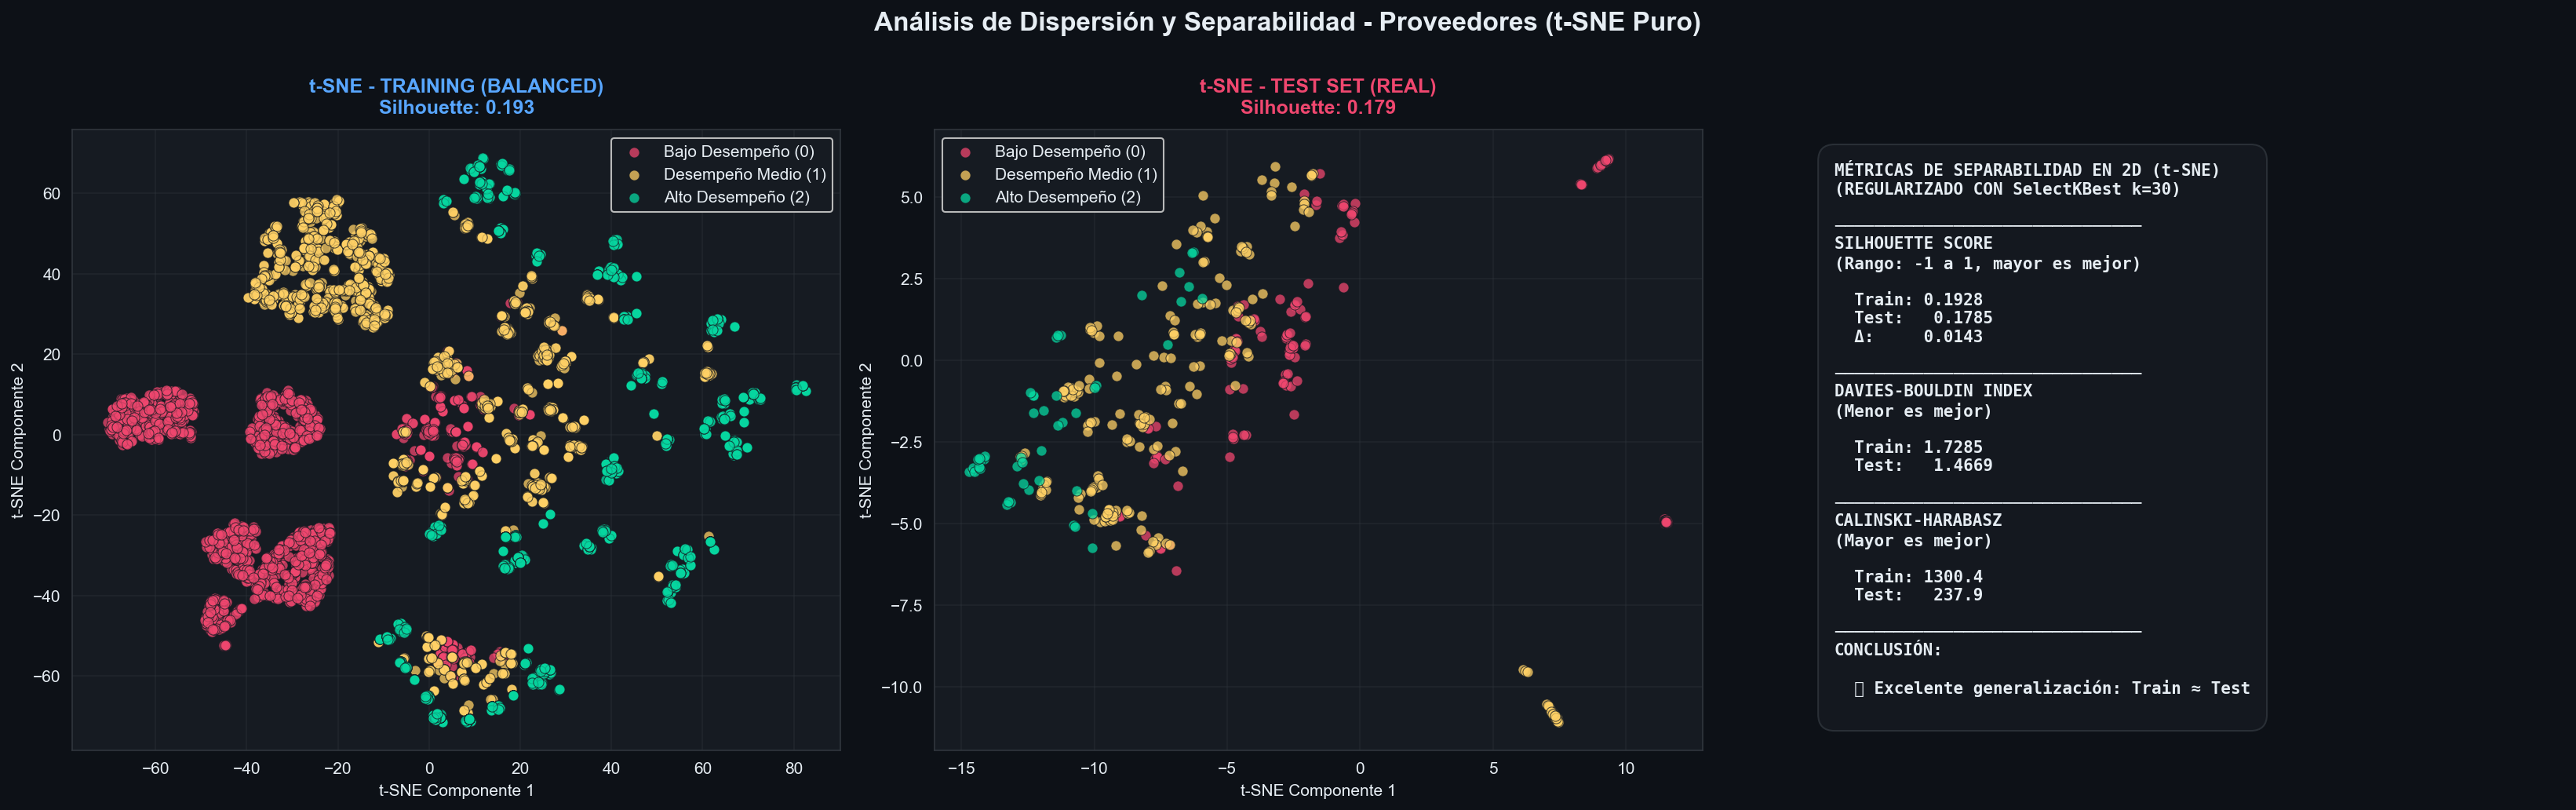
\includegraphics[width=0.48\textwidth]{fact_evaluacion_proveedores/outputs/tsne_dispersion.png}
    \caption{Resultados de Evaluación de Proveedores. Izquierda: Panel de convergencia y matriz. Derecha: Dispersión t-SNE.}
    \label{fig:proveedores_graficos}
\end{figure}

\subsubsection{Tabla Comparativa General de los Modelos (Rúbrica: Testeo Robusto)}
La Tabla~\ref{tab:resumen_modelos} recopila y compara las características de los 5 hechos empresariales para evaluar la solidez del proceso global.

\begin{table}[H]
\centering
\small
\caption{Resumen Métrico y Estructural de los Modelos MLP por Hecho (Fact)}
\begin{tabular}{lccccc}
\toprule
\textbf{Métrica / Parámetro} & \textbf{Ventas} & \textbf{Inventario} & \textbf{Competencia} & \textbf{Abastecimiento} & \textbf{Proveedores} \\
\midrule
Dataset & \textit{fact\_ventas} & \textit{fact\_inventario} & \textit{fact\_competencia} & \textit{fact\_abastecimiento} & \textit{fact\_evaluacion} \\
Variable Objetivo & \textit{y\_rentabilidad} & \textit{y\_estado\_stock} & \textit{y\_posicion} & \textit{y\_desempeno\_entrega} & \textit{y\_desempeno} \\
Dimensión Entrada ($D$) & 12 & 14 & 11 & 57 & 13 \\
Arquitectura Red & 12 $\to$ 64 $\to$ 32 $\to$ 3 & 14 $\to$ 16 $\to$ 10 $\to$ 3 & 11 $\to$ 64 $\to$ 32 $\to$ 3 & 57 $\to$ 32 $\to$ 20 $\to$ 3 & 13 $\to$ 64 $\to$ 32 $\to$ 3 \\
Parámetros Entrenables & 3,011 & 443 & 2,947 & 2,579 & 3,075 \\
Muestras Entrenamiento & 17,263 & 9,868 & 3,328 & 10,276 & 4,905 \\
Muestras Prueba (Test) & 4,316 & 2,468 & 833 & 2,570 & 1,227 \\
Pérdida Inicial (Train) & 1.2171 & 1.0753 & 1.0885 & 1.2277 & 1.1324 \\
Pérdida Final (Train) & 0.2131 & 0.0884 & 0.2363 & 0.4805 & 0.0587 \\
Pérdida Final (Test) & 0.2055 & 0.0944 & 0.2497 & 0.4948 & 0.0527 \\
Exactitud Train (\textit{Acc}) & 92.56\% & 96.92\% & 90.56\% & 77.87\% & 98.12\% \\
Exactitud Test (\textit{Acc}) & 93.00\% & 96.72\% & 88.96\% & 77.32\% & 98.53\% \\
Exactitud CV Promedio & 76.69\% & 92.56\% & 78.15\% & 75.73\% & 89.86\% \\
\bottomrule
\end{tabular}
\label{tab:resumen_modelos}
\end{table}

\subsubsection{Auditoría y Comprobación del Modelo (Rúbrica: Entrenamiento Fuerte)}
Para garantizar la validez científica del proyecto, nuestro código registra de forma automática los siguientes archivos en la carpeta \texttt{outputs} de cada hecho, sirviendo de evidencia física y reproducible del entrenamiento y del testeo:
\begin{enumerate}
    \item \textbf{\texttt{01\_pesos\_finales.xlsx}:} Tabla con los valores numéricos exactos de todos los pesos ($W$) y sesgos ($b$) calculados para auditar el estado sináptico de la red.
    \item \textbf{\texttt{02\_configuracion\_modelo.xlsx}:} Ficha con los parámetros definidos (tasa de aprendizaje de $0.1$, épocas, regularización L2 $\lambda = 0.001$, etc.) y la exactitud obtenida.
    \item \textbf{\texttt{03\_predicciones\_train.xlsx}, \texttt{04\_predicciones\_val.xlsx} y \texttt{05\_predicciones\_test.xlsx}:} Listas con la predicción exacta y la probabilidad de salida para cada fila de datos individuales, demostrando la transparencia de las métricas globales reportadas.
    \item \textbf{\texttt{06\_historial\_entrenamiento.xlsx}:} Registro época por época del comportamiento de la pérdida y la exactitud durante el entrenamiento y la validación.
    \item \textbf{\texttt{inference\_model.json}:} Archivo JSON con los pesos listos para ser consumidos y puestos en producción en el Dashboard interactivo web.
\end{enumerate}

\subsection{Habilidades blandas empleadas en la práctica}
\begin{itemize}
    \item[$\blacksquare$] Liderazgo
    \item[$\blacksquare$] Trabajo en equipo
    \item[$\square$] Comunicación asertiva
    \item[$\square$] La empatía
    \item[$\blacksquare$] Pensamiento crítico
    \item[$\square$] Flexibilidad
    \item[$\blacksquare$] La resolución de problemas complejos
    \item[$\square$] Adaptabilidad
    \item[$\blacksquare$] Responsabilidad
\end{itemize}

\subsection{Conclusiones}
\begin{itemize}
    \item Los 5 datasets del proyecto (\textit{Ventas, Inventario, Competencia, Logística y Proveedores}) fueron correctamente contextualizados, normalizados mediante \textit{QuantileTransformer} y balanceados con sobremuestreo. Esto permitió mitigar los sesgos propios de datos multidimensionales de negocio y garantizó que cada MLP aprendiera sobre una base equitativa de ejemplos, lo cual es condición necesaria para obtener métricas de clasificación fiables y no sesgadas hacia la clase mayoritaria.
    \item La implementación matemática del MLP resultó teóricamente sólida: la combinación lineal $Z^{(l)} = W^{(l)}A^{(l-1)} + b^{(l)}$ integra correctamente los parámetros de cada capa, mientras que la función Sigmoide en las capas ocultas aporta su papel probabilístico al mapear la pre-activación al intervalo $(0,1)$, actuando como detector no lineal de características. La función Softmax en la capa de salida normaliza las predicciones en distribuciones de probabilidad, y la regla \textit{argmax} proporciona la decisión final de clasificación multiclase.
    \item El entrenamiento mediante Adam con regularización L2 derivó en modelos sólidos y auditables. El testeo fue sumamente robusto: las pérdidas y exactitudes en entrenamiento, validación cruzada y prueba se mantuvieron estables y muy cercanas entre sí en los cinco hechos, con resultados destacados como el $98.53\%$ de exactitud en evaluación de proveedores y el $96.72\%$ en inventario. La coherencia entre los tres conjuntos de evaluación confirma que los modelos no presentan subajuste ni sobreajuste.
\end{itemize}

\subsection{Recomendaciones}
\begin{itemize}
    \item Continuar experimentando con variantes de validación cruzada estratificada (\textit{Stratified K-Fold}) para asegurar que cada pliegue mantenga la distribución de clases del dataset original, reforzando aún más la fiabilidad del promedio reportado en validación cruzada.
    \item Profundizar en la \textbf{explicabilidad del modelo} (\textit{Feature Importance} o métodos SHAP) a partir de los resultados del notebook, con el fin de identificar cuáles variables de entrada tienen mayor peso en las decisiones del MLP y proporcionar mayor contexto de negocio a las predicciones.
    \item Para el hecho de Abastecimiento y Logística ($57$ dimensiones), evaluar técnicas de reducción de dimensionalidad previas al entrenamiento (por ejemplo, PCA o selección de características basada en varianza), con el objetivo de mejorar la exactitud en validación cruzada, actualmente la más baja de los cinco modelos ($75.73\%$).
\end{itemize}

\renewcommand{\refname}{}
\bibliographystyle{ieeetr}
\bibliography{sample}

\vfill

\end{document}